\documentclass[a4paper,11pt]{article}

\usepackage{amsmath,amssymb,amsfonts,amsthm}    % Typical maths resource packages
\usepackage{graphicx}                           % Packages to allow inclusion of graphics
\usepackage{hyperref}                           % For creating hyperlinks in cross references
\usepackage[authoryear]{natbib}                 % literature reference style
\usepackage[bf]{caption}
\usepackage{bbm}
\usepackage{eurosym}
\usepackage{multirow}
\usepackage{pdflscape}
\usepackage{float}
\usepackage{dcolumn}
%\usepackage[colorinlistoftodos]{todonotes}
\usepackage{german}
\usepackage{color}
\definecolor{dkgreen}{rgb}{0,0.6,0}
\definecolor{gray}{rgb}{0.5,0.5,0.5}
\definecolor{mauve}{rgb}{0.58,0,0.82}
\definecolor{lightgray}{gray}{0.95}
\usepackage{listings}
\lstset{numbers=left,
	backgroundcolor = \color{lightgray},
	numberstyle=\tiny,
	numbersep=5pt,
	breaklines=true,
	showstringspaces=false,
	frame=l ,
	xleftmargin=15pt,
	xrightmargin=15pt,
	basicstyle=\ttfamily\scriptsize,
	stepnumber=1,
	keywordstyle=\color{blue},
  	commentstyle=\color{dkgreen},
  	stringstyle=\color{mauve}
}
\usepackage{caption}
\usepackage{dcolumn}

% -------------------------------
% --- some layout definitions ---
% -------------------------------

% define topline
\usepackage[automark]{scrpage2}
\pagestyle{scrheadings}
\automark{section}
\clearscrheadings
\ohead{\headmark}

% define citation style
\bibliographystyle{ecta}

% define page size, margin size
\setlength{\headheight}{1.1\baselineskip}
\voffset=-2cm
\hoffset=-3cm
\textheight24cm
\textwidth15.5cm
\topmargin1cm
\oddsidemargin3cm
\evensidemargin3cm

% define line line spacing = 1.5
\renewcommand{\baselinestretch}{1.25}

% define second level for `itemizing'
\renewcommand{\labelitemii}{-}
\newcommand{\E}{\mbox{I\negthinspace E}}

% Define new commands
\renewcommand{\figurename}{Figure}
\renewcommand{\tablename}{Table}
\renewcommand{\contentsname}{Table of Contents}
\renewcommand{\listfigurename}{List of Figures}
\renewcommand{\listtablename}{List of Tables}


\begin{document}
\lstset{language=R}
% -------------------------------
% --- frontmatter: Title page ---
% -------------------------------

\thispagestyle{empty}
\begin{center}
    {\LARGE{\bf Union Wage Effects in Germany - Implications for the Wage Distribution}} \vspace{1cm}


    {\large Seminar paper submitted\\\vspace{0.8cm}
    to}\\\vspace{0.5cm}
    {\large{\bf Alla Petukhina, Shi Chen and Niels Wesselh\"offt}} \\\vspace{0.8cm}
    {\large Humboldt-Universit\"at zu Berlin \\
    School of Business and Economics \\
    Ladislaus von Bortkiewicz Chair of Statistics} \vspace{1cm}


    {\large by \\\vspace{0.5cm}
    {\bf Felix B\"onisch, Nicole Hermann and Max Reinhardt}} \vspace{1cm}


    {\large in partial fulfillment of the requirements \\
    for the degree of \\
    {\bf Master of Science} \\\vspace{0.8cm}
    Berlin, August 18th, 2017}

\end{center}

% -----------------------------
% --- frontmatter: Contents ---
% -----------------------------
\newpage
\tableofcontents
\clearpage


% ----------------------------------------------------
% --- frontmatter: List of Figures (not mandatory) ---
% ----------------------------------------------------
\newpage
\pagenumbering{roman}
\addcontentsline{toc}{section}{List of Abbreviations}
\ohead[]{LIST OF ABBREVIATIONS}
\section*{List of Abbreviations}

\begin{tabular}{rp{0.2cm}lp{1cm}rp{0.2cm}l}
  CQPE      & & Conditional Quantile Partial Effect   & &    & &\\
  FC      & & Individual Coverage by Firm-Level Wage Bargaining Agreements  & &    & &\\
  GSES   & & German Structure of Earnings Survey   & &    & &\\
  IC      & & Individual Coverage by no Collective Contract   & &    & &\\
  IF      & & Influence Function   & &    & &\\
  OECD  & & Organization for Economic Cooperation and Development   & &    & &   \\
  OLS  & & Ordinary Least Squares   & &    & &   \\
  RIF      & & Recentered Influence Function   & &    & &\\
  SC      & & Individual Coverage by Sectoral Wage Bargaining Agreements   & &    & &\\
  shareFC      & & Share of Employees Covered by a Firm-Level Collective Contract within one Firm   & &    & &\\
  shareSC      & & Share of Employees Covered by a Sectoral Collective Contract within one Firm   & &    & &\\
  UQPE      & & Unconditional Quantile Partial Effect   & &    & &\\
\end{tabular}


% ----------------------------------------------------
% --- frontmatter: List of Figures (not mandatory) ---
% ----------------------------------------------------
\newpage
\addcontentsline{toc}{section}{List of Figures}
\ohead[]{\rightmark}
\listoffigures

% ---------------------------------------------------
% --- frontmatter: List of Tables (not mandatory) ---
% ---------------------------------------------------
\newpage
\addcontentsline{toc}{section}{List of Tables}
\listoftables


% -------------------------------
% --- main body of the thesis ---
% -------------------------------
\newpage
\pagestyle{plain}
\setcounter{page}{1}    % start page numbering anew
\pagenumbering{arabic}  % page numbers in arabic style


\section{Introduction}
The existence of labor market unions is certainly one of the major departures from the market wage-setting mechanism. By utilizing their bargaining power and restricting labor supply, unions may achieve above market wages. Moreover, the union bargaining results affect wage dispersion, because wages are attached to jobs rather than to employees \citep{Bryson:14}. However, the size and quality of union wage effects depend on a variety of factors such as the bargaining power of unions, the institutional level of collective bargaining and the factors included in the bargaining process, all of which make it a heavily contested field of research.

In this paper we will estimate the effect of collective bargaining coverage on mean wages for covered employees in Germany using a linked employer-employee dataset, the German Structure of Earnings Survey (GSES) 2010. Then, conditional and unconditional quantile regressions are employed in order to estimate the effect of collective bargaining on wage dispersion. Throughout the theoretical considerations and our econometric investigation, we distinguish between individual coverage on the sectoral and firm-level as well as the within-firm collective bargaining coverage ratio for both collective bargaining regimes.

It proves important to distinguish between union density and collective bargaining coverage. Union density refers to the share of employees that are unionized, whereas collective bargaining coverage comprises all employees that are covered by a collective agreement. As can be seen in figure \ref{Fig:UDandCC2}, union density and collective bargaining coverage can greatly differ from one another within one country. In addition, there is a declining trend in trade union density as well as collective bargaining coverage. Whereas union density rose in Spain, it decreased in all other OECD countries, that are included in figure \ref{Fig:UDandCC2}, from 1990 to the latest year recorded.\footnote{Please see appendix B Figure \ref{Fig:UDandCC2} for a breakdown of the country-specific latest years of record.} The OECD average of collective bargaining coverage declined as well, with disproportionately high losses in countries with lower coverage ratios in 1990.

The institutional landscape of unions varies across countries, affecting the gap between union density and collective bargaining coverage. Employees may be covered by sectoral wage bargaining agreements, which are negotiated between an employer's association and an employee union. A second possible form of coverage is firm-level coverage, which results from bargaining between a single firm and an employee union. In Germany, these two forms of bargaining are mutually exclusive. In the United States, for example,  bargaining predominantly takes place at the firm-level and union density and the share of covered employees are relatively similar (Fig. \ref{Fig:UDandCC2}). Conversely, in Germany and other European countries, bargaining is primarily conducted at the sectoral level and the coverage rate generally exceeds union density (Fig. \ref{Fig:UDandCC2}). International differences in the institutional setup and country-specific legal settings explain the disparities between collective bargaining coverage and union density. For example, in France and Spain, employers are not allowed to discriminate against non-union members, compared to unionized employees. Therefore, collective contracts have to be extended to non-union members and as a result collective coverage exceeds union density. This depicts a free-rider problem with regard to union membership and explains the low rates of union density relative to collective coverage in some countries. In countries where discrimination between unionized and non-unionized employees is legal, such as the United States (US) and the United Kingdom (UK), union density is considerably higher relative to collective coverage. In Germany, employers often voluntarily extend collective contracts to non-unionized workers. Following from the German Collective Bargaining Act,\footnote{ Tarifvertragsgesetz} collective contracts have to be applied to a specific job match, only if the employer is part of an association and the employee is a member of a union. Hence, the extension is not forced by law, but a response to the bargaining power of employees \citep{Fitzenberger&Kohn&Lembcke:13}. However, there is some room for deviation since employers are always free to pay higher wages than collectively negotiated (favorability principle). Furthermore, individual wages of covered employees may differ as each employee has the right not to associate, according to the German constitution.\footnote{ negative Koalitionsfreiheit}

The results of our econometric investigation show a positive union wage effect of individual coverage for low-wage earners under both coverage regimes. The effect declines along the wage distribution and eventually turns negative for high-wage earners, which indicates a compression of the wage distribution. Furthermore, an increase in the share of covered employees increases wages in the firms that apply either sectoral or firm-level contracts.

The aim of this paper is to present an empirical paper with the use of the statistical programming language R. The paper is organized as follows. Section \ref{Sec:Data} provides information of the raw data. Section \ref{Sec:Data_Prep} is a process to improve the quality of the data information and to put raw data into the form so that we can work scientifically with these data. In this section we will carry out some standardization of the variables, as well as transformations and calculations of new variables. Section \ref{Sec:Des_Stat} shows how to display tables and graphics using own functions. In order to analyze the above-described economic relations, we are using different regression analysis methods in section \ref{Sec:regressionR}. Then in section \ref{Sec:Conc} the statistical programming results are summarized.

\section{Dataset}\label{Sec:Data}

In order to analyze the effect of union coverage on wages and wage dispersion, we use the \emph{German Structure of Earnings Survey 2010}. Data for the GSES is collected since 1951 and periodically every 4 years since 2006. The cross-sectional linked employer-employee dataset includes information for public sector as well as private sector employers and employees. After German law,\footnote{ Verdienststatistikgesetz} employers have an obligation to provide the requested information, preventing a selection bias in the data and making it more reliable. In the data collection process, the method of stratified sampling was used: Initially, some 34,000 firms with ten or more employees were selected based on the federal state, the branch of economic activity and the size of the firm, keeping the sample as representative as possible. In a second step, about 1,9000,000 employees from the selected firms were randomly chosen.

The dataset contains information on individual employee characteristics (sex, age, education,...), on occupation (years in firm, industy,...) and on earnings (gross and net income, income tax,...). Moreover, the GSES 2010 provides information on union coverage, not only on the firm-level, but more importantly also on an individual level. That enables us to determine the shares of employees within a firm, covered by a union regime.

For our analysis we use the scientific-use file provided by the Research Data Centers of the Federal Statistical Office and the statistical offices of the L\"ander. Scientific-use files do not have to be used at the Research Data Center, but in return the data is anonymized in a way that prevents firms and individuals from being possibly identified. The anonymization has repercussions on the potential of the econometric analysis as some firm and individual characteristics are left out or considerably generalized. For example, all municipalities are grouped into five regions, branches of economic activity are consolidated, the number of employees in a firm is summarized into three categories and annual gross pay is top-coded for values larger than \euro 750.000. Regarding union coverage, the coverage regime is only indicated if three or more firms within one industry and region apply a sectoral or firm-level agreement, leading to a loss of roughly 300.000 observations. 

Since we use a large data set, it is necessary to clean the working space before loading the data file by using the function \texttt{rm (list = ls ())}. If the data is loaded into R, we get a raw data set of 1,890,418 observations and 52 variables. A complete listing of the variables can be found in the appendix tables \ref{raw1} and \ref{raw2} , the following table \ref{var} lists only the part of the variables that are used more often in our econometric investigation. Table \ref{var} results from simple functions such as \texttt{mean()}, \texttt{summary()}, \texttt{as.data.frame()} and other useful functions provided by R to view data. Some variables have missing values, which are encoded as NA. Different levels are encoded with a number e.g. variable \texttt{ef\$10} contains information about the gender of respondents which has only two characteristics (levels) either male (\texttt{ef\$10 == 1}) or female (\texttt{ef\$10 == 0}). The same procedure is used for other nominal variables. In order to see which numeric encodings do the levels have, it is sufficient to look at the Min and Max columns from table \ref{var} and the order of the listed levels from corresponding command \texttt{a.data.frame(summary())}.

\begin{landscape}
\begin{table}[p]
\scriptsize
\centering
\caption{Variables used in later econometric investigation}
\label{var}
\begin{tabular}{|l|l|l|l|l|l|l|l|}
\hline
\textbf{Variable} & \textbf{Label}                                 & \textbf{Level of measurement} & \textbf{Obs} & \textbf{Mean} & \textbf{Std. Dev.} & \textbf{Min} & \textbf{Max} \\ \hline
ef9               & Performance group for compensation             & nominal                       & 1.593.794    & NA            & NA                 & 1            & 5            \\ \hline
ef10              & Gender (male==1, female==2)                    & nominal                       & 1.890.418    & NA            & NA                 & 1            & 2            \\ \hline
ef16u2            & Education                                      & nominal                       & 1.890.418    & NA            & NA                 & 1            & 7            \\ \hline
ef40              & Work experience in years                       & ratio                         & 1.890.222    & 10,9071       & 11,25833           & 0            & 45           \\ \hline
ef41              & Age in years                                   & ratio                         & 1.890.222    & 41,37514      & 12,44701           & 16           & 66           \\ \hline
ef9be             & Involvement of public in the company's capital & nominal                       & 1.408.474    & NA            & NA                 & 1            & 2            \\ \hline
ef12be            & Share of female workers in the firm            & ratio                         & 1.890.418    & 43,67534      & 31,94675           & 0            & 100          \\ \hline
ef26be            & Number of the employees of the enterprise      & ratio                         & 1.890.418    & 1290,626      & 3482,053           & 1            & 44523        \\ \hline
\end{tabular}

\end{table}
\end{landscape}



\section{Data Preparation}\label{Sec:Data_Prep}
The goal of the data preparation part is to bring the data in form which can be later used for the descriptive statistics as well as the regression analysis part. This section contains two quantlets which are stated below. The main part of the first quantlet is to build a function which calculates the respondents per company. The second quantlet produces variables to indicate how many employees per company are covered by a union contract or not. In both quantlets we generate dummy variables, which are necessary for carrying out the regression analysis.

\subsection{Implementation}
First we calculate how many respondents exist per company. To determine this we create a general function which can be applied on other data sets with similar structure, since the function takes a vector as input value which contains the information on which employee belongs to which company. The function is called with the following command:
\lstset{firstnumber = 31}
\begin{lstlisting}
respond = respondFunc(dat$ef1)
\end{lstlisting}
For explaining the function code we use a small example. Assume we have the following simplified data set containing only five employees and the company they belong to:
\begin{table}[h!]
\centering
\caption{Example Data 1}
\label{ex1}
\begin{tabular}{|l|l|}
\hline
observation & company \\ \hline
1           & 1       \\ \hline
2           & 1       \\ \hline
3           & 2       \\ \hline
4           & 2       \\ \hline
5           & 3       \\ \hline
\end{tabular}
\end{table}
\newline
The function \texttt{respondFunc} creates a vector called \texttt{respond} with the length of the data vector passed into the function. In our example from table \ref{ex1} the vector has the length of five:
\lstset{firstnumber = 19}
\begin{lstlisting}
 respond = numeric(length(dat))
\end{lstlisting}
After setting the counting variables to one we create an auxiliary variable \texttt{temp}. In \texttt{temp} the frequency of every variable of the giving data vector is stored by using the R integrated function \texttt{table}:
\lstset{firstnumber = 22}
\begin{lstlisting}
 temp = table(dat) 
 \end{lstlisting}
Applying the function to our small example we obtain an absolute frequency table:
 \begin{table}[h!]
\centering
\caption{Output \texttt{table}}
\label{my-label}
\begin{tabular}{|l|l|}
\hline
company & frequency \\ \hline
1       & 2         \\ \hline
2       & 2         \\ \hline
3       & 1         \\ \hline
\end{tabular}
\end{table}

Furthermore we integrate a \texttt{for loop} in our function which goes through all observations and saves the number of respondents per company for each company. Again we demonstrate this procedure in our small example. The \texttt{for loop} is stated out below:
\lstset{firstnumber = 23}
\begin{lstlisting}
for (i in 1:length(dat)){                 
    j = dat[i]                           
    respond[i] = temp[j]                  
    i = i+1              
  } \end{lstlisting}
In our example the \texttt{for loop} would work five times as we have five employees. The value of the first employee e.g. in which company the first employee is working is stored in \texttt{j}. Then the function accesses the \texttt{j}th element of \texttt{temp} and stores the information in the \texttt{i}th element of \texttt{respond}. Since \texttt{temp} stores the number of employees per company we obtain following result for our example:
\begin{table}[h!]
\centering
\caption{Result \texttt{respondfunc} example}
\label{my-label}
\begin{tabular}{|l|l|l|}
\hline
observation & company & respondents per company \\ \hline
1           & 1       & 2                       \\ \hline
2           & 1       & 2                       \\ \hline
3           & 2       & 2                       \\ \hline
4           & 2       & 2                       \\ \hline
5           & 3       & 1                       \\ \hline
\end{tabular}
\end{table}


For further investigation we need several dummy variables Therefore we create al function to create dummy variables since this procedure is for most of the dummy variables the same. The function takes two values as input variables:
\lstset{firstnumber = 43}
\begin{lstlisting}
dummyFunc = function(dat , x)
\end{lstlisting}
The \texttt{dat} will be the information vector and the \texttt{x} will be one level which will be compared to the vector. The function itself contains only one line of code:
\lstset{firstnumber = 40}
\begin{lstlisting}
 d = as.numeric(dat == levels(dat)[x])      
  return(d)
}
\end{lstlisting}
In line 40 we use the implemented function in R called \texttt{as.numeric} together with a comparison. The \texttt{as.numeric} function converts a \texttt{TRUE} value into ones and a \texttt{FALSE} value in zeros. The first dummy variable which needed to be created is dummy for east and west. If the dummy is zero that means the employee is working in a company in west Germany. This is done be the function call shown below:
\lstset{firstnumber = 45}
\begin{lstlisting}
east = dummyFunc(dat$ef4be , 5)
dat["east"] = east       
\end{lstlisting}
The dummy variable \texttt{east} is added to the data frame at the end. Using this function we have to pay attention to the levels we want to do the comparison inside the function. The next dummy we create is a dummy for education. Therefore we use our function \texttt{dummyFunc}. Moreover we reduce the number of different dummies from six to three by simple addition of two dummies which we want to combine. The whole procedure is stated out below:
\lstset{firstnumber = 49}
\begin{lstlisting}
tempEdu1  = dummyFunc(dat$ef16u2 , 1 )
tempEdu1a = dummyFunc(dat$ef16u2 , 2 )
tempEdu2  = dummyFunc(dat$ef16u2 , 3 )
tempEdu2a = dummyFunc(dat$ef16u2 , 4 )
tempEdu3  = dummyFunc(dat$ef16u2 , 5 )
tempEdu3a = dummyFunc(dat$ef16u2 , 6 )
tempNa    = dummyFunc(dat$ef16u2 , 7 )
tempNa[tempNa == 1] = NA                

educ1 = tempEdu1 + tempEdu1a + tempNa
educ2 = tempEdu2 + tempEdu2a + tempNa
educ3 = tempEdu3 + tempEdu3a + tempNa

dat["educ1"] = educ1                   
dat["educ2"] = educ2
dat["educ3"] = educ3  
\end{lstlisting}
In line 55 and line 56 we convert the missing values from the data. Line 66 to 68 shows the calculation of the dummies. The same procedure is applied by creatig dummies for employees with a permanent contract.
For creating a dummy variable for employees working in shifts we use a different comparison. That is why we cannot use our function described before:
\lstset{firstnumber = 72}
\begin{lstlisting}
shift        = as.numeric(dat$ef23 >= 1)
dat["shift"] = shift                       
\end{lstlisting}
The statement in line 72 evaluates to 1 if the compared value is larger or equal to 1. Using similar approach we create a dummy for employees working full-time and reduce dimension. In this case we cannot use our pre-defined function as the comparison is different.
\lstset{firstnumber = 76}
\begin{lstlisting}
tempFull1 = as.numeric(dat$ef16u1 != "Teilzeitbeschaeftigt - Beamter")
tempFull2 = as.numeric(dat$ef16u1 != "Teilzeitbeschaeftigt - weniger als 18 Std.")
tempFull3 = as.numeric(dat$ef16u1 != "Teilzeitbeschaeftigt - 18 Std. und mehr")
fulltime  = tempFull1+tempFull2+tempFull3 - 2
dat["fulltime"] = fulltime         
\end{lstlisting}
We get ones for all values of \texttt{dat\$ef16u1} which do not match with the chosen level. In line 79 the addition is done. We have to subtract the dummy by 2 to get a normal zero and one dummy variable. The next dummy variable we create shows whether a worker gets the minimum wage or not. The calculation procedure is the same as before and is not stated out again:
\lstset{firstnumber = 83}
\begin{lstlisting}
minimumWage   = as.numeric(dat$ef31be != "nein")
minimumWageNa = dummyFunc(dat$ef31be , 3 )
minimumWageNa[minimumWageNa == 1] = NA           #add NA's from dataset
minimumWage        = minimumWage+minimumWageNa
dat["minimumWage"] = minimumWage + minimumWageNa 
\end{lstlisting}


The second part of the data preparation is done below. We build a \texttt{contractFunc} and create new variables later used for our regression analysis. In this part we calculate how many employees per company have a collective bargaining agreement and if they have a collective bargaining agreement. We distinguish between individual contract and firm wide contract. Our function has three input parameters:
\lstset{firstnumber = 91}
\begin{lstlisting}
contractFunc = function(a,b,c){   
\end{lstlisting}
The \texttt{a} is the company dummy. It shows to which company each employee belongs to. The \texttt{b} is the information vector filled with the dummies which sais if the employee has collective bargaining agreement or not and if the employee has one. It distinguishes between individual contract and firm wide contract. With the input \texttt{c}  we choose the level. In our case we have three different options as already stated out. As this function is a more complex function we use the example data to explain the method (see table \ref{ex2}):
\newline
\begin{table}[h!]
\centering
\caption{Example Data 2}
\label{ex2}
\begin{tabular}{|l|l|l|}
\hline
observation & company & contract \\ \hline
1           & 1       & 1 = no contract        \\ \hline
2           & 1       & 1        \\ \hline
3           & 1       & 2 = individual contract       \\ \hline
4           & 2       & 2        \\ \hline
5           & 2       & 3 = firm wide contract       \\ \hline
6           & 2       & 3        \\ \hline
7           & 2       & 1        \\ \hline
8           & 2       & 2        \\ \hline
9           & 3       & 1        \\ \hline
10          & 3       & 1        \\ \hline
\end{tabular}
\end{table}
\newline
\lstset{firstnumber = 96}
\begin{lstlisting}
temp = table(a)
cumtemp = cumsum(temp)                   
cumtemp = append(cumtemp,0,after =0)    
\end{lstlisting}
First we use an integrated function \texttt{table} to calculate how many different employees we have per company and store its value in \texttt{temp}. Then in line 97 the cumulated sum is calculated using the function \texttt{cumsum}. This is done for correct storing of the results later as the frequency on how many people have a collective bargaining agreement or not will be calculated for each company. For a correct starting value we need to add zero as the first value which is done in line 98.The result would have following output:
\newline
\begin{table}[h!]
\centering
\caption{Output \texttt{table} 2 and cumulated sum}
\label{my-label}
\begin{tabular}{|l|l|l|}
\hline
company & frequency & cumulated \\ \hline
        &           & 0         \\ \hline
1       & 3         & 3         \\ \hline
2       & 5         & 8         \\ \hline
3       & 2         & 10        \\ \hline
\end{tabular}
\end{table}
\newline
After those calculations the main part of the function is stated out below:
\lstset{firstnumber = 100}
\begin{lstlisting}
 g = nrow(temp) +1
  i = 2                                   
  j = 1
  k = 1
  q = numeric(length(b))
  for (i in 2:g){
    k = cumtemp[i-1]+1                    
    j = cumtemp[i]                         
    p = table(b[k:j])                     
    q[k:j]  = p[c]                   
    i = i+1
  }
  return(q)
}   
\end{lstlisting}
Some initializations of different counting variables are done and are not further commented. In the initializations of the \texttt{for loop} you can see that it will loop over every company in the data set (there is a total of 32220 companies in the data set). In \texttt{k} will be stored the $i-1$ value of the cumulated sum. Which will be the first employee of company x. If we would have not appended the zero in line 98 we would leave out the first company. In line 107 the last employee of company x is stored in \texttt{j}. In line 108 we use the function \texttt{table} again and apply on the data vector passed on to the function on the before calculated sector (e.g. company x from \texttt{k} to \texttt{j}). The result of \texttt{table} is then stored in \texttt{p}. Then we store the information of \texttt{p} with the chosen level in \texttt{q} in line 109. As an output for our example we get:
\begin{table}[h!]
\centering
\caption{Output after running the loop}
\label{label}
\begin{tabular}{|l|l|l|l|l|}
\hline
observation & company & no contract & indivdiual contract & firm wide contract \\ \hline
1           & 1       & 2           & 1                   & 0                  \\ \hline
2           & 1       & 2           & 1                   & 0                  \\ \hline
3           & 1       & 2           & 1                   & 0                  \\ \hline
4           & 2       & 1           & 2                   & 2                  \\ \hline
5           & 2       & 1           & 2                   & 2                  \\ \hline
6           & 2       & 1           & 2                   & 2                  \\ \hline
7           & 2       & 1           & 2                   & 2                  \\ \hline
8           & 2       & 1           & 2                   & 2                  \\ \hline
9           & 3       & 2           & 0                   & 0                  \\ \hline
10          & 3       & 2           & 0                   & 0                  \\ \hline
\end{tabular}
\end{table}

The calculations for our three different levels is then done with three functions calls. After the calculation the values are stored in the data frame as well:
\lstset{firstnumber = 116}
\begin{lstlisting}
noTariff = contractFunc(dat$ef1, dat$ef8, 1)
SCTariff = contractFunc(dat$ef1, dat$ef8, 2)
FCTariff = contractFunc(dat$ef1, dat$ef8, 3) 
dat["noTariff"] = noTariff                
dat["SCTariff"] = SCTariff
dat["FCTariff"] = FCTariff
\end{lstlisting}
The next step was to create shares on how many employees per company have an individual contract (line 125) and also for firm wide contracts (line 124). The calculated values are then stored again in the data frame:
\lstset{firstnumber = 124}
\begin{lstlisting}
shareFC = FCTariff/respond
shareSC = SCTariff/respond
dat["shareFC"] = shareFC            
dat["shareSC"] = shareSC
\end{lstlisting}
We need dummy variables for the different collective bargaining agreements. We use our already explained function \texttt{dummyfunc} for generating the dummies:
\lstset{firstnumber = 130}
\begin{lstlisting}
noTariffDummy = dummyFunc(dat$ef8 , 1)
SCTariffDummy = dummyFunc(dat$ef8 , 2)
FCTariffDummy = dummyFunc(dat$ef8 , 3)
\end{lstlisting}
Then we create interaction terms which we need later for our regression analysis:
\lstset{firstnumber = 138}
\begin{lstlisting}
shareFCFC = shareFC*FCTariffDummy
shareSCSC = shareSC*SCTariffDummy
\end{lstlisting}
We need for our regression analysis two variables age squared and experience squared:
\lstset{firstnumber = 144}
\begin{lstlisting}
agesq = dat$ef40*dat$ef40
expsq = dat$ef41*dat$ef41
\end{lstlisting}
The last step in the data preparation part is to calculate the individual wage per employee and the $log$ wage. We set all values where the denominator was zero in line 150 to \texttt{NA} so we do not get any infinity values in our data set:
\lstset{firstnumber = 150}
\begin{lstlisting}
wage   = ifelse(dat$ef18+dat$ef20 == 0, NA, 
	(dat$ef21+dat$ef22)/(dat$ef18+dat$ef20))
lnWage = log(wage)
\end{lstlisting}

\subsection{Testing}

The testing procedure for our code is not so easy because the code is written for a specific data set. It still makes sense when a researcher gets his data set updated frequently and he needs to apply a certain data preparation procedure over and over again. He can write a program like we did and can then always apply the code to the new data set without changing the code.
However if this code is used by other person it would be helpful to think about possible errors. We included therefore error messages in our functions. In our first function called \texttt{respondFunc} we implemented some error messages for missing data and wrong data input:
\lstset{firstnumber = 17}
\begin{lstlisting}
  if (missing(dat))
    stop("No data passed to the function")
  if (is.numeric(dat)!= TRUE)
    stop("numeric data needed")                       
\end{lstlisting}
The first error message proof is a data vector was included in the function header. The second error message shows up when data is passed to the function which is not numeric. The error messages are quite basic due to the fact that the code requires a specific data set as already stated out. In our second function \texttt{dummyFunc} we use similar error messages except the one where we check if any levels are existing in the vector which basically means it is not a dummy variable.
\lstset{firstnumber = 38}
\begin{lstlisting}
 if (missing(dat))
    stop("No data passed to the function")
  if(is.null(levels(dat)))
    stop("No levels found")                   
\end{lstlisting}

In the second quantlet we implemented three error message in the function which are similar to those from the \texttt{respondFunc}:
\lstset{firstnumber = 92}
\begin{lstlisting}
  if (missing(b))
    stop("No data passed to the function")
  if (is.numeric(a)!= TRUE & is.numeric(b)!= TRUE  )
    stop("numeric data needed")
  if (missing(c))
    stop("No level selected")
  if (c > sum(nlevels(b)))
    stop("Selected level to large")  
\end{lstlisting}
First we check if data is passed to the function or not and if a level is selected. The last error message shows up if a level is selected which is to large. In the following code in quantlet two we apply already explained function \texttt{dummyFunc} and do simple calculations. Calculating the wage we have to pay attention of possible error due to a denominator which could be zero. This would yield to infinity values in our data set. We took care of this problem by simply setting zero values to \texttt{NA}.

\subsection{Conclusion}
Considering functionality given the specific data set our code from the first quantlet works good. It is helpful as already pointed out when a researcher gets a updated data set frequently. On the other side the \texttt{respondFunc} could be more complex also taking for example data in form of table 4 as input. The \texttt{dummyFunc} could be more complex allowing for different comparison method inside the function (line 40) then just the is equal (\texttt{==}) comparison. Our function forms a foundation and can be further modified if the data sets become more complex, which was not necessary in our case.

The conclusion of our second quantlet is similar to the first one since the second quantlet is a part of the data preparation and the same function is used partially. Again the function \texttt{contractFunc} could be more complex since it can only handle numeric dummies. The function could be modified in a way that it takes names of different contracts as dummy variables. As we already took care of possible infinity values the code can be seen as as sufficiently robust.
\section{Descriptive Statistics}\label{Sec:Des_Stat}

Descriptive statistics is an important part of data analysis. Many contexts can be represented by simple graphs and tables. In addition, the descriptive statistics provide a good visualization of the data, as an ancient Chinese proverb says; one picture is worth a thousand words. In this chapter, we will focus on how to build tables and graphs with predefined settings using our own functions. Functions that we have built in this section can be used through customizations by others and is easy to replicate. In the following section the code of 3 quantlets is described and discussed.

\subsection{Implementatition}

In this section we want to show some implementation of R to build tables and graphs. Moreover we focus on variables which are economically important for the regression analysis. The first glance is on the age distribution of the population and the possibly prevailing differences in gender. An appropriate graph for visualizing age distribution is the population pyramid. To plot population pyramid in R, we use the \texttt{plotrix} package, which must be installed before.
\lstset{firstnumber = 157}
\begin{lstlisting}
install.packages("plotrix")
library("plotrix")
\end{lstlisting}
In order to use the plot function \texttt{pyramid.plot} from the \texttt{plotrix}-package we have to calculate the relative frequencies of age distribution according to the gender. Therefore we constructed a function \texttt{frequency}.
\lstset{firstnumber = 161}
\begin{lstlisting}
frequency = function(k, l){
  100*sweep(table(k,l), 2, colSums(table(k,l)), "/")
}
\end{lstlisting}
Function \texttt{frequency} calculates a table with frequencies of the variable k with different characteristics which are given in l. In our case we determine k as the age variable \texttt{dat\$ef41} and l as gender \texttt{dat\$ef10}. Function \texttt{frequency} uses sweep function and relies on summary statistics such as colSum for calculating relative frequancies of different age of male and female subjects, this results in following table:
\begin{table}[h!]
\centering
\caption{Frequency table generated by the function \texttt{frequency(dat\$ef41, dat\$ef10)}}
\label{freq}
\begin{tabular}{l|c|c|}
\cline{2-3}
                                 & \multicolumn{2}{c|}{\textbf{l}} \\ \hline
\multicolumn{1}{|l|}{\textbf{k}} & männlich       & weiblich       \\ \hline
\multicolumn{1}{|l|}{16}         & 0.2446         & 0.1777         \\ \hline
\multicolumn{1}{|l|}{17}         & 0.5249         & 0.4334         \\ \hline
\multicolumn{1}{|l|}{18}         & 0.8379         & 0.7812         \\ \hline
\multicolumn{1}{|l|}{...}        & ...            & ...            \\ \hline
\multicolumn{1}{|l|}{66}         & 1.2839         & 0.8838         \\ \hline
\end{tabular}
\end{table}

The function \texttt{buildpopulation} was generated to produce and simultaneously save the population pyramid graphic in a separate pdf file. Such functions are very useful especially if you want to create a lot of similar plots, which should always have the settings to look uniform. However, such settings can be permanently defined in the function or can also be defined as a freely selectable variable.
\lstset{firstnumber = 170}
\begin{lstlisting}
buildpopulation = function(k, l, popname){
  pop = frequency(k, l)
  pdf(popname)
  	pyramid.plot(pop[,1], pop[,2], labels = rownames(pop), gap = 2, lxcol = "blue", rxcol = "red")
  dev.off()
}
\end{lstlisting}
The function \texttt{buildpopulation} uses variables k and l which are neccessary for the \texttt{frequency} function and popname for setting a name for the graphic such as \glqq populationpyramid.pdf\grqq{}. Within the function \texttt{buildpopulation} the results of the \texttt{frequency} function are assigned to an auxiliary variable pop. This merely serves for a better overview in the further use of the generated results of the \texttt{frequency} function in the \texttt{pyramid.plot} and is not absolutely necessary. Since we are interested in union wage effects, we therefore investigate the age distribution of the union covered population and a population without any union contract. Therefore we generate a subsample with a data which include only union covered workers such as:
\lstset{firstnumber = 183}
\begin{lstlisting}
datFCSC = dat[ which(FC == 1 | SC == 1),]
\end{lstlisting}
Starting from the subsample we can finally build the population pyramid using the function \texttt{buildpopulation}. The same approach is used for the population pyramid for workers without a union contract. Defining such subsample we have to ensure that the worker neither covered by on sectoral collective nor firm contract (\texttt{.which(FC == 1 | SC == 1)}). 
\lstset{firstnumber = 189}
\begin{lstlisting}
buildpopulation(datFCSC$ef41, datFCSC$ef10, "populationFCSC.pdf")
\end{lstlisting}
This results in the following two graphics: 

\begin{minipage}[t]{0.475\textwidth}
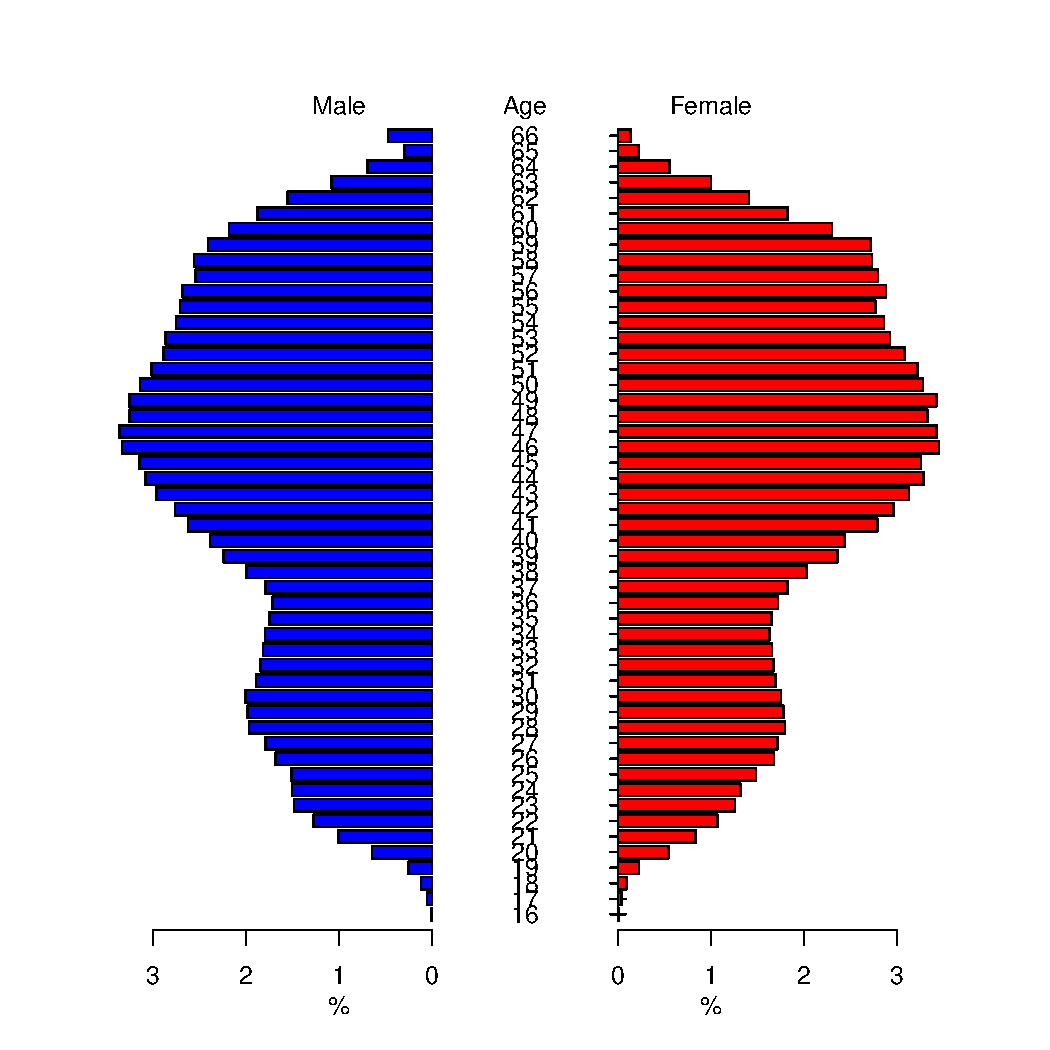
\includegraphics[width=\textwidth]{populationFCSC}
\captionof{figure}{Population pyramid of employees covered by a union contract}
\label{fig:popFCSC}
\end{minipage}
%\hfill
\begin{minipage}[t]{0.475\textwidth}
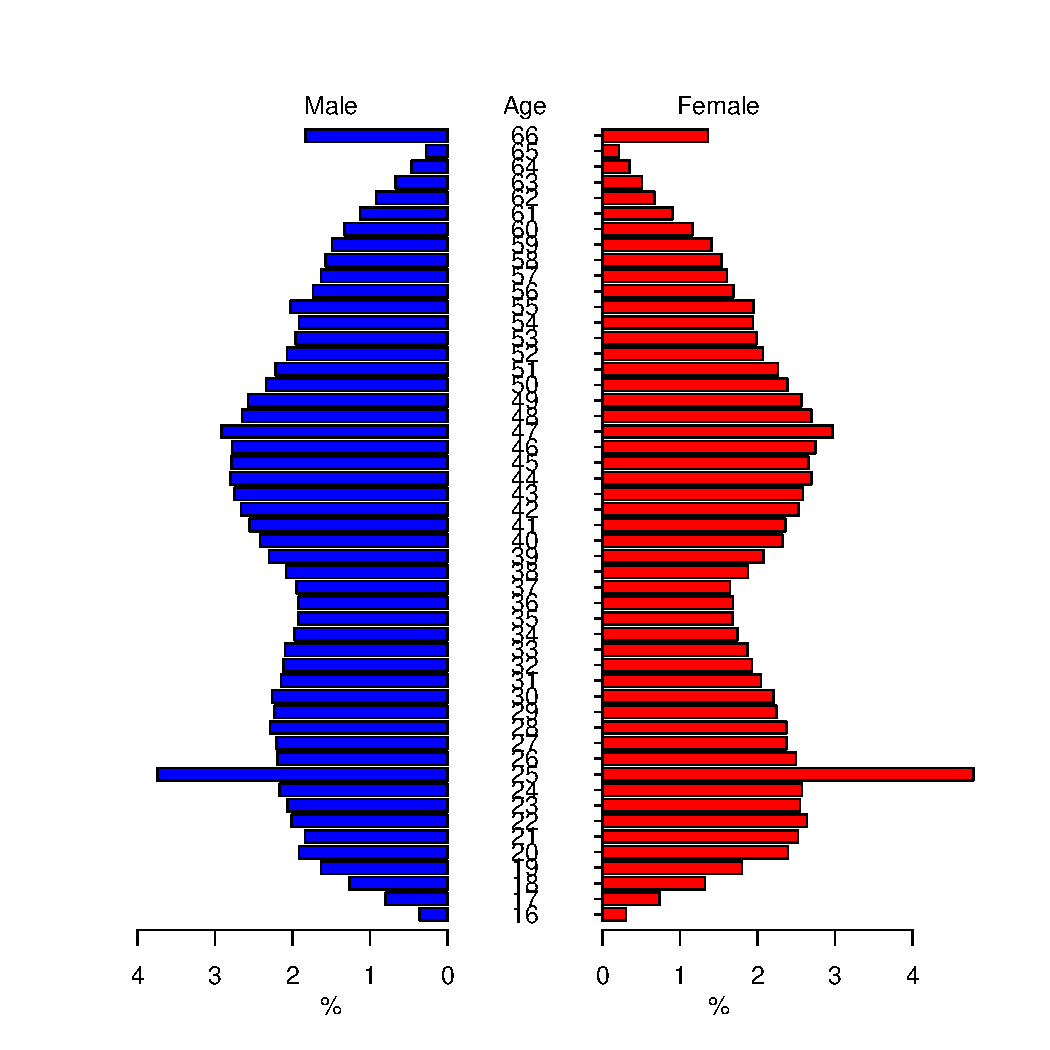
\includegraphics[width=\textwidth]{populationNoFCSC}
\captionof{figure}{Population pyramid of employees not covered by a union contract}
\label{fig:popNoFCSC}
\end{minipage}
\vspace{0.5cm}


Due to the visualisation of the data by the population pyramid, there are no recognizable differences in the age structure between man and woman in both subsamples. However, the general age distribution in the group of workers with a union contract differs from the workers without. Population with a union contract seems to be older than the population without. To fix this statement numerically, we calculate the median. Indeed the average age of the workers with a trade union contract is 45 years, while the average age of the workers without a union contract is 40.

The function \texttt{buildboxplot} was created following a similar principle to the function \texttt{buildpopulation}, which generates and saves the graphic in a pdf file.
\lstset{firstnumber = 208}
\begin{lstlisting}
buildboxplot =  function (v, w, boxname, z){
  pdf(boxname, width = 11, height = 7)
  boxplot(v~w, range=2.5, width=NULL, notch=FALSE,varwidth=FALSE, names = z,
          boxwex=0.8, outline=FALSE, staplewex=0.5, horizontal=FALSE, border="black",
          col="#94d639", add=FALSE, at=NULL)
  abline(h = median(v, na.rm = TRUE), col = "red")
  dev.off()
}
\end{lstlisting}

Function \texttt{buildboxplot} uses four characteristics: v, w, boxname and z. V is a numeric variable and w is a group variable into which the numeric variable v will be splitted. Using boxname we can predetermine the name of the file such as \glqq boxplot\_ lnwage\_ education.pdf\grqq{}. Z is a vector with label names of the group variable w, so that the length of the vector z agrees with the number of the levels in w. Within the \texttt{buildboxplot} function we insert into the boxplot a red line which characterises the median of the numeric variable v in the investigated population.
\lstset{firstnumber = 240}
\begin{lstlisting}
buildboxplot(data$lnwage, data$ef16u2, "boxplot_lnwage_education.pdf", educLAB)
\end{lstlisting}
The results of the \texttt{buildboxplot} function are shown in the figure \ref{Fig:boxplot}.
\begin{figure}
\begin{center}
\caption{Boxplot of education differences in ln(Wage)}
\label{Fig:boxplot}
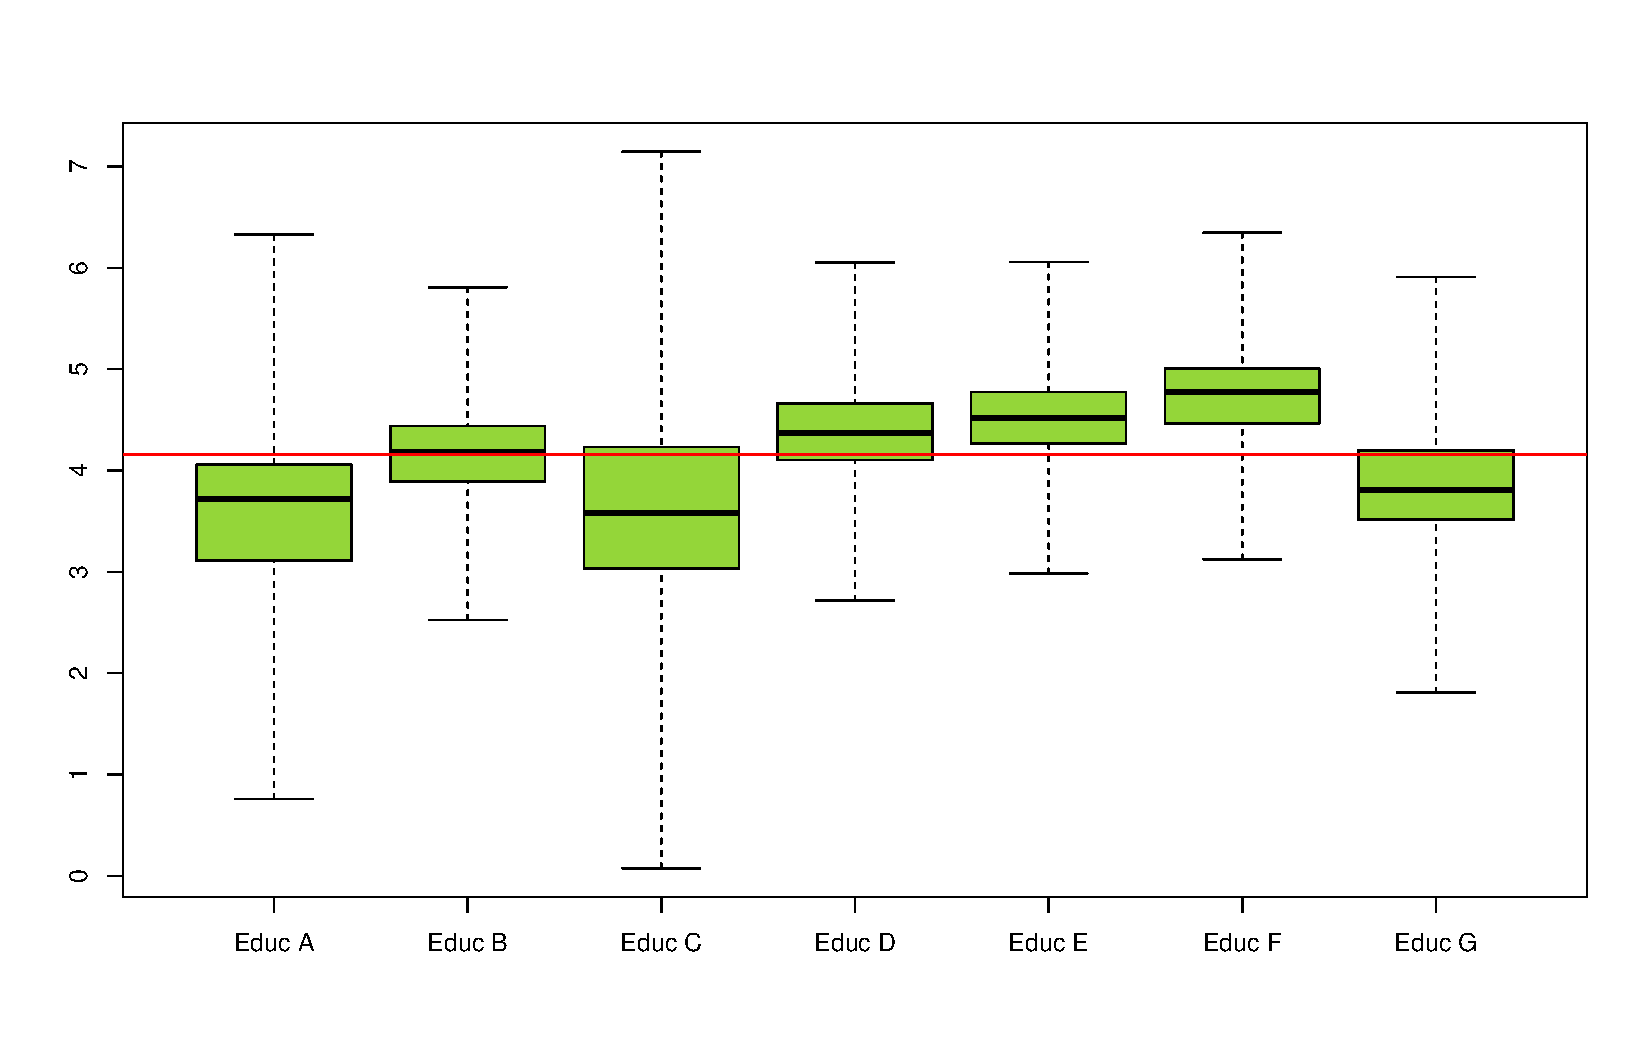
\includegraphics[scale=0.55]{boxplot_lnwage_educ}
\end{center}
\end{figure}
The figure \ref{Fig:boxplot} shows ln(Wage) distribution over different education levels. Education level \texttt{educLab} results following characteristics:
\begin{itemize}
\setlength\itemsep{0em}
\item \textbf{Educ A:} Middle school without vocational training;
\item \textbf{Educ B:} Middle school with vocational training;
\item \textbf{Educ C:} High school without vocational training;
\item \textbf{Educ D:} High school with vocational training;
\item \textbf{Educ E:} Professional university degree;
\item \textbf{Educ F:} University degree;
\item \textbf{Educ G:} Education unknown.
\end{itemize}
The higher the level of education of the worker the higher the median wage in this education group. This is in line with the basic theory of human capital. A middle school and high school education leads to higher wages when a vocational training has been completed afterwards (compare groups Educ A and C with Educ B and D). By using the subsamples, we can again create two graphs with workers with union contract and workers without.\footnote{Please see appendix B Figures \ref{Fig:educFCSC} and \ref{Fig:educNoFCSC} for a comparison of the wages distribution over different education level in different subsamples.} The workers with union contract earn on average more than those without. But also the wage distribution in the same education group differs strongly in the subsamples. While the wage distribution in the subsample with union contract is more homogenous, there is a large variation in the subsample with workers without a union contract especially in groups with a lower education level.

In this part we will present the functions used in our quantlet 4. Functions \texttt{quant} and \texttt{buildquantileplot} are made to examine correlations between two numeric variables along the quantiles e.g. the effect of work experience along the wage distribution. First we build a function \texttt{quant(x,y,q)} for calculating quantiles. Along the variable x the function calculates for every $x_{i}$ a quantile q of the variable y. The vector q consists of the quantiles we want to investigate and can be changed as desired. The vector color must have the same number of elements as the vector q, since each q is assigned a color.
\lstset{firstnumber = 255}
\begin{lstlisting}
  quant = function(x,y,q){
                  aggregate(x, y, na.rm=TRUE, quantile, q)
  }

  q = c(0.10, 0.25, 0.50, 0.75, 0.90)
  color = c("orange", "red", "green", "blue", "black")
\end{lstlisting}
Using the quantiles which are aggregated by the function \texttt{quant}, we can build a scatterplot with the quantile lines. Therefore we build a function \texttt{buildquantileplot} which contains a simple scatterplot of the independent variable x and dependent variable y. Using \texttt{xla} and \texttt{yla} we can add labels to a plot and using \texttt{plotname} determine the name of the pdf file. Such scatterplot can be applied to any problems where the quantile distribution maybe different. It is  useful graph to have a look to quantile distribution of a numeric variable and could be helpful to state an appropriate regression method.
\lstset{firstnumber = 277}
\begin{lstlisting}
buildquantileplot = function(x, y, xla, yla, plotname){
  pdf(plotname)
  #plot points
  plot(x, y, ylim=c(2,8), pch = 1, col='dark green',
       xlab = xla, ylab = yla)
  #plot quantilelines
  for (l in 1:length(q)){
    lines(quant(y, list(x), q[l]), col = color[l], lwd =2)
  }
  dev.off()
}
\end{lstlisting}
Using the \texttt{for loop}, we add the quantile lines to the scatterplot, the quantiles already defined in q.
\lstset{firstnumber = 303}
\begin{lstlisting}
buildquantileplot(datNoFCSC$ef40, datNoFCSC$lnwage, "Experience", "Ln(wage)",
		  "scatterplot_lnwage_experience_NoFCSC.pdf")
\end{lstlisting}
After executing the function \texttt{buildquantileplot} with the dependent variable ln(wage) (\texttt{dat\$lnWage}) and independent variable experience (\texttt{dat\$ef40}). The following graph demonstrates relation between the wages and work experiances along different wage quantiles, which we will analyse in more detail below using the quantile regression.
\begin{figure}
\begin{center}
\caption{Effect of work experiences along the wage distribution}
\label{Fig:scatter}
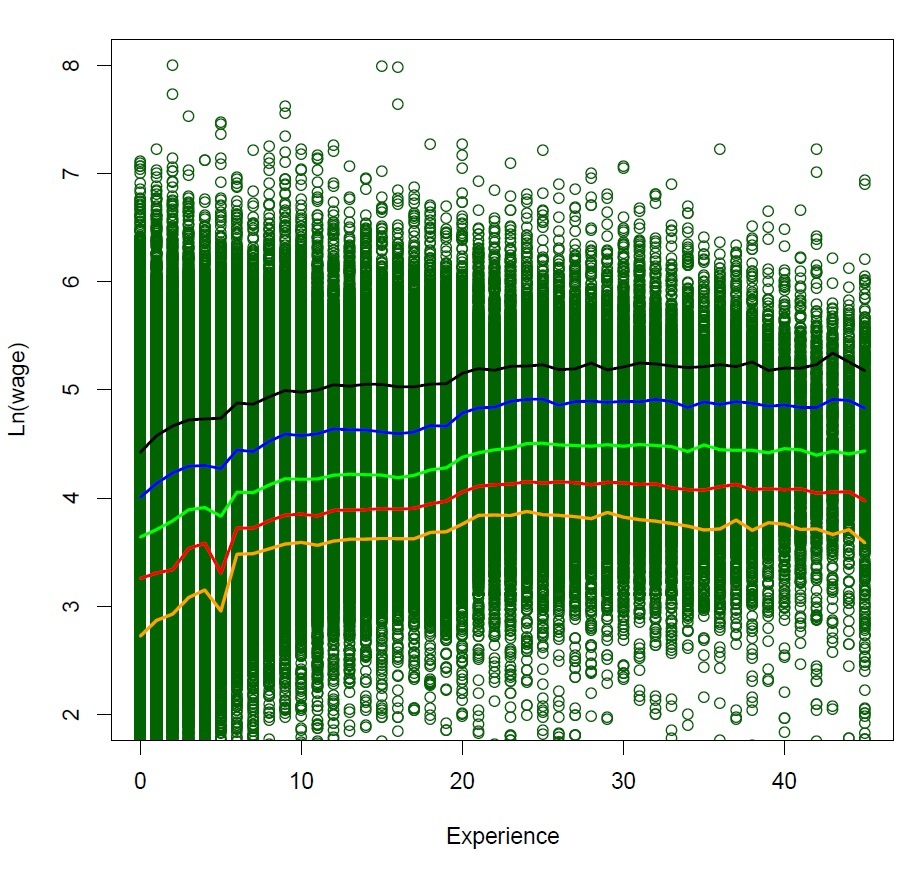
\includegraphics[scale=0.4]{scatterplotNoFCSC-lnwage-experience}
\end{center}
\end{figure}
The quantile lines in the scatterplot of the subsample with the workers without a union contract have all the same positive trend but different slopes. Therefore the quantile regression seems to be more appropriate than the ordinary least square approach. Nevertheless, this statement is subjective and will be examined in the section \ref{Sec:Regression}.

We distinguish between three different union bargaining regimes:\\
\noindent\hspace*{6mm} (SC) refers to a sectoral collective contract, which is negotiated between employer's associations and employee unions,\\
\noindent\hspace*{6mm} (FC) refers to a firm contract, which is negotiated between an employee's union and a single firm, and\\
\noindent\hspace*{6mm} (IC) refers to contracts, individually negotiated between employee and employer. And we extend the econometric analysis to female employees in order to be able to make statements regarding the gender wage gap at mean wages and across quantiles. The challenge of the following part namely our quantlet 5 is to create a table with the information stated above. Such a table shall contain the mean and the standard deviation  of the hourly log wages and the share of different union contracts.
Since those calculations in a data frame are time-consuming in case of large data, we convert first the data frame into a data table. Therefore we install  neccessary package and put it into our local \texttt{R} library:
\lstset{firstnumber = 319} 
\begin{lstlisting}
dat = data.table(dat)             
\end{lstlisting}
The variable \texttt{Group} is created by using the three dummy variables which are labled in \texttt{Group} as 1: SC , 2: FC and 3: IC. Excluding all \texttt{NA}'s we generate the number of observations according to the new variable \texttt{Group}, which is neccessary for further calculation of the $\log$ mean wage and the standard deviation for each group and each gender.
\lstset{firstnumber = 330} 
\begin{lstlisting}
sum = dat[!is.na(Group), .N]                                 
\end{lstlisting}
Following code shows how to order the results by gender:
\lstset{firstnumber = 333} 
\begin{lstlisting}
lnWageSummary = dat[!is.na(Group), .(LogHourlyWageMean = mean(lnWage, na.rm = T),         
                                     LogHourlyWageSD = sd(lnWage, na.rm = T)), by = .(ef10, Group)]  
lnWageSummary = lnWageSummary[order(ef10, Group)]                                   
\end{lstlisting}
Exactly the same procedure will be done for overall population. Using the \texttt{table} function we generate the absolute frequencies of SC, FC and IC devided by gender.
\lstset{firstnumber = 347} 
\begin{lstlisting}
mtable = table(dat$Group, dat$ef10)                                            
\end{lstlisting}
The same approach is applied to construct employee share and order it by \texttt{Group}. The already existing results are packed into a table in the following step where we use the \texttt{prop.table} function to provide the proportion of the employees of different level of the variable \texttt{Group} and for female and male subjects:
\lstset{firstnumber = 356} 
\begin{lstlisting}
lnWageSummaryTotal = data.frame(Regime       = c("SC", "FC", "IC"),                                   
                     MaleEmpolyeeShare       = prop.table(mtable, 2)[, 1],  
                     MaleLogHourlyWageMean   = lnWageSummary[ef10 == "maennlich", LogHourlyWageMean],    
                     MaleLogHourlyWageSD     = lnWageSummary[ef10 == "maennlich", LogHourlyWageSD],       
                     FemaleEmpolyeeShare     = prop.table(mtable, 2)[, 2],                             
                     FemaleLogHourlyWageMean = lnWageSummary[ef10 == "weiblich", LogHourlyWageMean],                            FemaleLogHourlyWageSD   = lnWageSummary[ef10 == "weiblich", LogHourlyWageSD],     
                     TotalEmpolyeeShare      = TotalEmpolyeeShare$Share,                                                        TotalLogHourlyWageMean  = lnWageSummaryOverall$LogHourlyWageMean,                
                     TotalLogHourlyWageSD    = lnWageSummaryOverall$LogHourlyWageSD,                                            stringsAsFactors        = FALSE)                                          
\end{lstlisting}
The calculation and creation of the row \texttt{total} is similar to the first part and not further commented in the quantlet 5. Created vector \texttt{total} is added to the data frame \texttt{lnWageSummaryTotal}. Few corrections using some basic R functions can make the output much more readable. Using function \texttt{rapply} we transform all numbers into a numeric value and round the results by setting \texttt{digit} to 2.
\lstset{firstnumber = 401} 
\begin{lstlisting}
lnWageSummaryTotal[,2:10] = rapply(lnWageSummaryTotal[,2:10], as.numeric)
lnWageSummaryTotal        = rapply(object = lnWageSummaryTotal, f = round, classes = "numeric", how =       "replace", digits = 2)
\end{lstlisting}
At the end of the quantlet the data which was temporary stored in the data table format is transformed back into a data frame. R provides a very useful package \texttt{xtable}, which makes it possible to print the table in a tex-file. This is a great advantage of R compared to other software. It allows the scientist to transfer the results smoothly into the report paper. Above all, it is useful and requires little effort if the data change. 
\lstset{firstnumber = 405} 
\begin{lstlisting}
dat = data.frame(dat)   
install.packages("xtable")
library(xtable)
print(xtable(lnWageSummaryTotal, type = "latex"), file = "covRegimeandLNWages.tex")
\end{lstlisting}

Table \ref{Coverage Regime} summarizes the shares of coverage regime affiliations as well as mean log wages for male and female employees under the different bargaining regimes in the GSES 2010 sample. $33\%$ of male employees ($37\%$ of female employees) are covered by a sectoral contract and $6\%$ of both male and female employees are covered by contracts negotiated on the firm-level. These figures are lower than the coverage ratios obtained by \cite{Fitzenberger&Kohn&Lembcke:13} in their analysis of the 2001 data. The literature confirms, that this is due to a decline in collective coverage in recent years \citep{Addison&Bryson&Teixeira&Pahnke6Bellmann:13}. A possible explanation for the discrepancy is that the sample of employees is not representative for the population. The proportion of employees in the sample from large firms compared to all employees in large firms is lower than the proportion of employees from smaller firms.
\begin{table}[h]
\scriptsize
\centering
\caption{Coverage Regime Affiliation and Log Wages for Male and Female Employees}
\label{Coverage Regime}
\begin{tabular}{l|ccccccccccc}
\multicolumn{4}{c}{male}                                                                               & \multicolumn{3}{c}{female}             &\multicolumn{3}{c}{overall}                                                              \\
\hline
\multirow{2}{*}{regime} & \multirow{2}{*}{employee-share} & \multicolumn{2}{l}{log hourly wages}    & \multirow{2}{*}{employee-share} & \multicolumn{2}{l}{log hourly wages}    & \multirow{2}{*}{employee-share} & \multicolumn{2}{l}{log hourly wages}\\
                        &                       & mean    & std. dev.   &                                         & mean           & std. dev.         &                   & mean           & std. dev.          \\
\hline
SC                      &     $0.33$     &   $4.34$     &   $0.47$   &                       $0.37$           &   $4.24$     &   $0.41$                             &$0.35$&$4.29$& $0.44$\\
FC                      &     $0.06$     &   $4.41$     &   $0.41$   &                       $0.06$           &   $4.24$     &   $0.34$                             &$0.06$& $4.33$& $0.39$\\
IC                      &     $0.61$     &   $4.08$     &   $0.73$   &                       $0.57$           &   $3.81$     &   $0.61$                             &$0.59$& $3.97$& $0.69$\\
total                   &     $1.000$     &   $4.19$     &   $0.65$   &                       $1.00$           &   $4.01$     &   $0.56$                            &$1.00$& $4.11$& $0.62$\\
\hline
\end{tabular}
\end{table}
Mean log hourly wages are highest among employees with firm-specific collective contracts. Employees under firm-specific coverage earn more on average than employees having individually negotiated their contract, suggesting that there is a union wage premium. Moreover, women earn less than men regardless of the coverage regime. Concluding from the standard deviation figures, wage dispersion is highest among employees, not covered by a collective agreement and higher among male employees.

\subsection{Testing}

The section \ref{Sec:Des_Stat} consists of 3 quantlets and 5 own functions. In order to use the functions correctly by others, following control command is implemented in each function:
\lstset{firstnumber = 162} 
\begin{lstlisting}
  if (missing(k))
    stop("No data passed to the function. Variable k has to be determined.")
\end{lstlisting}
In the first line we check if the variable necessary for the execution of the function is missing. If it is missing, an error message is displayed stating that a variable must still be determined to execute the function. We have installed this error message in each of our functions for each variable.

In the second part of the error messages the numeric variables are checked explicitly. We can explain this by the examples of the functions \texttt{frequency} and \texttt{quant}. The function \texttt{frequency (k, l)} uses the variable k and l, in which case no variable must necessarily be a numerical variable since only the relative frequencies are calculated. Let's look at a concrete example: \texttt{frequency(dat$ef16u2, dat$ef10)}. We execute the function \texttt{frequency()} with two non numeric variables: education and gender. Indeed our function calculates the relative frequencies. Note that the sum over the one column is 100\%. If we want to check in advance whether a variable is numeric, we execute the command \texttt{is.numeric()}. If the variable is numeric then we get the value \texttt{TRUE} otherwise \texttt{FALSE}. The function \texttt{quant(y, x, q)} again uses three variable and two of them must be numeric. This applies to the variables \texttt{y} and \texttt{q}. Variable \texttt{q} defines the quantile to be calculated, which can be either a number like \texttt{q = 0.5} (also called median) or a vector \texttt{q = c (0.25, 0.5, 0.75)}. Variable y must be numeric because the quantile is calculated for this variable. For this reason, the following error messages are installed in the function quant:
\lstset{firstnumber = 262} 
\begin{lstlisting}
  if (is.numeric(y) != TRUE)
    stop("Numeric data needed. y has to be numeric")
  if (is.numeric(q) != TRUE)
    stop("Numeric data needed. Quantile q was wrong specified.
    q can be either a number or a numeric vector.")
\end{lstlisting}

Our \texttt{buildpopulation} and \texttt{buildquantileplot} functions call up other functions such as \texttt{quant} and \texttt{frequency}, so the error messages which were already executed in the implemented \texttt{quant} and \texttt{frequency} functions are no longer implemented in the new code of the function e.g. \texttt{buildpopulation} to avoid redundancy.

Furthermore in functions \texttt{buildpopulation}, \texttt{buildboxplot} and \texttt{buildquantileplot}, the name of the pdf file is defined in the function header. At the end of the name of the file \texttt{.pdf} must be attached, the entire expression must be specified in quotation marks, and only then plots are built correctly and stored in an external pdf file. If the name is not entered correctly, an error message from R will appear automatically. For example, lets call the function \texttt{buildpoulation(dat\$ef41, dat\$ef10, \"populationFCSC.pdf\")}. This is the correct execution of the function. Let's delete the quotes: \texttt{buildpoulation (dat$ef41, dat$ef10, populationFCSC.pdf)}. Then following error message appears:\\ \texttt{\textcolor{red}{Error in gsub(\dq \%\textbackslash \%\dq , \dq \dq , s) : object \dq populationFCSC.pdf\dq not found}}.\\This means that the pdf file cannot be created because the entered name does not have the correct syntax. Since this error message is already a component in R, it is not possible for us to modify it and to adapt it specifically to our example.
% 
The code of quantlet 5 cannot be really tested as it is specific for our given problem how to calculate the wanted table. One can test the result by using a calculator which would take rather long as we have over $1.5$ million observations or when you work in a team another person can calculate the same table in a different way and compare the results at the end. As we calculated only mean, standard deviation and the shares there are not many sources for errors because those values are almost all calculated by internal functions. Errors could occur from wrongly selected columns in the data table. But these errors are often easy to identify.


\subsection{Conclusion}

The functions of the quantlets created for the descriptive statistic are efficient and can be easily applied to other issues. The functions fulfill their purpose and make the code much more compact and clear. Especially the function quant can show us differences in median and quantiles between groups, which is very useful when comparing groups and when choosing variables for regression.\footnote{ Example: When calling \texttt{quant(dat\$ef41, dat\$ef9, 0.5)}, we can immediately calculate the medians of the variable ages in the different employee groups.} An advantage of construction table \ref{Coverage Regime} is that the calculation is done easily and fast. By using the \texttt{data.table} package the calculation is even faster because the package can handle big data sets easily. Some disadvantages are if you want to export your table into a \texttt{.tex} file you are not as flexible in the layout as when you are doing it just in latex.


\section{Regression Analysis}\label{Sec:regressionR}
In order to analyze the effects of union coverage on wages and the wage distribution we will use three different econometric frameworks. Firstly, we will employ an OLS regression to investigate the effect on mean wages. However, the OLS regression framework of exploring the determinants of wages does not account for the possibility that covariates may have differential impacts across various parts of the wage distribution. Instead of focusing on the effect of union coverage on mean wages, the quantile regression approaches allow us to analyze the effects on different quantiles of the wage distribution. Hence, we can determine the contribution of union coverage to wage dispersion.

\subsection{OLS}
\subsubsection*{Theory}
We are interested in the effect of union coverage on wages. Let $ Y $ denote the outcome variable hourly wage and $ F_y(y) $ its distribution function, where $ F_y(y)=Pr(Y\leq y) $. $ X $ determines the union coverage status of one of the two union regimes (firm-level or sectoral-level) and is therefore a dummy variable, $ x= \{0,1\}$. $ Y_1 $ and $ Y_0 $ can be denoted as the possible outcomes under alternate values of $ X $. Hence, $Y=X\cdot Y_1 + (1-X)\cdot Y_0$, if union coverage is statistically independent of the possible outcomes. The unconditional distribution function for Y can be expressed as a weighted average of conditional distribution function of Y given X, weighted by the unconditional distribution of X \citep{Borah&Basu:2013}:

\begin{equation}\label{1}
  F_{y}(y)=Pr(X=1)F_{Y|X}(y|X=1) + Pr(X=0)F_{Y|X}(y|X=0)
\end{equation}

The ordinary least squares estimator gives us a consistent estimator of the target parameter $\beta_{OLS}$, that measures the effect of a marginal change in $X$ on the conditional expectation of $Y$, $\beta_{OLS}=\E[Y|X=1]-\E[Y|X=0]$. However, in most cases, useful interpretations can only be drawn from the effect of a change in the unconditional distribution of $X$ on the unconditional distribution of $Y$. One convenient feature of the OLS estimator is, that it is a consistent estimator for the effect on the unconditional distribution of $Y$ as well,\footnote{ This holds true as long as the estimated model is linear in all parameters.} because:
\begin{equation}\label{2}
  \E [Y]=p(X)\E[Y|X=1]+(1-p(X))\E[Y|X=0]
\end{equation}
\begin{equation*}
  \frac{d\E[Y]}{dp(X)}=\E[Y|X=1]- \E[Y|X=0]=\beta_{OLS}
\end{equation*}

Therefore, the coefficients obtained by OLS regression can be interpreted as the effect of a marginal change of $X$ on the unconditional mean of $Y$.

\subsubsection*{Implementation}
First, we are installing the package \texttt{dplyr} in order to be able to select specific cells in the data frame. The \texttt{stargazer} package allows us to construct a table as \LaTeX -output, summarizing the regression results.
\lstset{firstnumber = 416}
\begin{lstlisting}
install.packages("dplyr")
library(dplyr)
install.packages("stargazer")
library(stargazer)
\end{lstlisting}
The regression of log hourly wages is done with respect to a set of covariates $ X \equiv [I, F, V] $, where $ I $ represents individual worker characteristics, such as education, years in the firm, gender and full-time working status. Firm characteristics are denoted by $ F $ and include, but are not limited to region and the share of female employees. $V$ refers to a vector of union coverage variables, containing (i) dummy variables for sectoral (SC) and firm-level (FC) coverage, (ii) variables for the share of employees within a firm, covered by either sectoral (shareSC) or firm-level (shareFC) collective contracts and (iii) interaction effects. The resulting regression can be expressed as:
\begin{equation}\label{OLS equation}
\begin{split}
   ln(w_{kn})= &  \beta_{0}+I_{kn}\beta_{X}+F_{n}\beta_{F} \\
   & +SC_{kn}\beta_{SC}+FC_{kn}\beta_{FC}+ shareSC_{n}\beta_{shareSC} +shareFC_{n}\beta_{shareFC}\\
   &  +SC_{kn} \cdot shareSC_{n}\beta_{shareSCxSC}+FC_{kn}\cdot shareFC_{n}\beta_{shareFCxFC} \\
\end{split}
\end{equation}
\begin{center}with $k=1,\dots , K$ individual employees and $n=1,\dots , N$ firms.\end{center}
In particular, we employ 4 different specifications of the regression model with different sets of wage bargaining indicators (\texttt{model1},..., \texttt{model4}, see quantlet 6. The \texttt{lm()} function is used to carry out the regression with \texttt{lnWage} being mentioned first as the dependent variable and all following variables as the explanatory variables, using the data set \texttt{dat}.
\lstset{firstnumber = 421}
\begin{lstlisting}
#OLS regression with 4 different specifications
model1 = lm (lnWage ~ FCTariffDummy + SCTariffDummy + ef10 + east + ef9be + ef12be + ef26be + minimumWage + ef9 + educ2 + educ3 + shift + ef40 + agesq + ef41 + expsq + permanent , dat )
\end{lstlisting}
Using the \texttt{stargazer} package, we are generating a table, that summarizes the regression results of \texttt{model1, model2, model3, model4} line 431 in a single table. The option \texttt{keep} allows us to create a vector of covariates, whose coefficients we want to display in the table. For a better understanding, the labels are changed, using the option \texttt{covariate.labels}. The other options allow us to align the output at the decimal mark in the \LaTeX -output (\texttt{align}), omit the results for the F-statistic and standard error of regression (\texttt{omit.stat}), remove empty lines from the table (\texttt{no.space}) and determine the file name (\texttt{out}).
\lstset{firstnumber = 430}
\begin{lstlisting}
#output table result in latex code
stargazer(model1, model2, model3, model4, title="Results OLS Regression" ,
          keep = c("FCTariffDummy", "SCTariffDummy", "shareFC" , "shareSC" , "shareFCFC" , "shareSCSC" , "ef10") ,
          covariate.labels=c("Firm Contract","Sectoral Contract", "share FC","share SC","shareFCxFC","shareSCxSC" , "gender (male = 0)"),
          align=TRUE , omit.stat=c("ser","f"),  no.space=TRUE, out = "olsregression.tex")
\end{lstlisting}
% Table created by stargazer v.5.2 by Marek Hlavac, Harvard University. E-mail: hlavac at fas.harvard.edu
% Date and time: Fri, Aug 18, 2017 - 10:11:02 AM
% Requires LaTeX packages: dcolumn
\begin{table}[!htbp] \centering
  \caption{Results OLS Regression}
  \label{OLSresults}
\begin{tabular}{@{\extracolsep{5pt}}lD{.}{.}{-3} D{.}{.}{-3} D{.}{.}{-3} D{.}{.}{-3} }
\\[-1.8ex]\hline
\hline \\[-1.8ex]
 & \multicolumn{4}{c}{\textit{Dependent variable:}} \\
\cline{2-5}
\\[-1.8ex] & \multicolumn{4}{c}{lnWage} \\
\\[-1.8ex] & \multicolumn{1}{c}{(1)} & \multicolumn{1}{c}{(2)} & \multicolumn{1}{c}{(3)} & \multicolumn{1}{c}{(4)}\\
\hline \\[-1.8ex]
 Sectoral Contract & 0.044^{***} &  & -0.053^{***} & 0.062^{***} \\
  & (0.001) &  & (0.002) & (0.003) \\
  Firm Contract & 0.058^{***} &  & -0.116^{***} & 0.060^{***} \\
  & (0.001) &  & (0.004) & (0.008) \\
  share SC &  & 0.044^{***} & 0.134^{***} & 0.218^{***} \\
  &  & (0.001) & (0.002) & (0.003) \\
  share FC &  & 0.070^{***} & 0.217^{***} & 0.313^{***} \\
  &  & (0.002) & (0.005) & (0.006) \\
  shareSCxSC &  &  &  & -0.212^{***} \\
  &  &  &  & (0.005) \\
  shareFCxFC &  &  &  & -0.294^{***} \\
  &  &  &  & (0.011) \\
  gender (male = 0) & -0.075^{***} & -0.071^{***} & -0.073^{***} & -0.073^{***} \\
  & (0.001) & (0.001) & (0.001) & (0.001) \\
 \hline \\[-1.8ex]
Observations & \multicolumn{1}{c}{700,886} & \multicolumn{1}{c}{848,798} & \multicolumn{1}{c}{700,886} & \multicolumn{1}{c}{700,886} \\
R$^{2}$ & \multicolumn{1}{c}{0.586} & \multicolumn{1}{c}{0.587} & \multicolumn{1}{c}{0.589} & \multicolumn{1}{c}{0.591} \\
Adjusted R$^{2}$ & \multicolumn{1}{c}{0.586} & \multicolumn{1}{c}{0.587} & \multicolumn{1}{c}{0.589} & \multicolumn{1}{c}{0.591} \\
\hline
\hline \\[-1.8ex]
\textit{Note:}  & \multicolumn{4}{r}{$^{*}$p$<$0.1; $^{**}$p$<$0.05; $^{***}$p$<$0.01} \\
\end{tabular}
\end{table}
\subsubsection*{Results}


The results of the OLS regression are presented in table \ref{OLSresults}. The regression results include a full set of firm-specific and individual covariates as well as different sets of union coverage variables. Specification (1) only includes the dummy variables for sectoral and firm-level collective coverage and suggests a union wage premium of $4.4\%$ for employees covered by a sectoral contract compared to employees without any collective bargaining contract. The union wage premium for employees under firm-level contracts is estimated to be even higher at $5.8\%$. Both effects are significant at the $1\%$-level.

Specification (ii) is restricted to the effect of the shares of covered employees within a firm on log wages. It turns out, that a $10\%$ increase in the share of covered employees within a firm yields on average a $0.44\%$ increase in wages for employees under sectoral collective coverage, and a $0.70\%$ increase for employees under a firm-level contract, respectively. Again, both effects are significant at the $1\%$ level.

In specification (iii), dummy variables for sectoral and firm-level coverage on an individual level as well as the firm-level coverage shares (shareSC and shareFC) are included. The individual coverage regime effects turn negative, whereas a higher share of covered employees in a firm is still associated with higher wages. In fact, the effects of higher coverage shares on wages increased to $1.34\%$ for a $10\%$ increase in the share of employees covered by a sectoral agreement ($2.17\%$ for a 10\% in crease in the share of employees covered by a firm-level agreement). Therefore, in a firm with close to $0\%$ coverage, union wage premiums turn negative. Conversely, in a firm with full coverage, the union wage premium is positive ($-0.053+100\% \cdot 0.134=0.081$ under sectoral contracts and $-0.116 +100\% \cdot 0.217=0.101$ under firm-level contracts).

Interaction effects between individual coverage and the share of covered employees in a firm are introduced in specification (iv). The individual coverage coefficients turn positive again and the effect of an increasing share of covered employees within a firm rises as well, compared to the other specifications. However, the interaction effects are estimated to be negative, suggesting that in firms with low coverage, individual coverage leads to higher wages than in firms with high coverage. The effect of individual coverage by a sectoral collective contract (firm-specific contract) in a firm with an average coverage ratio is $-1.2\%$\footnote{ $\beta_{SC}+\overline{shareSC}\cdot \beta_{shareSCxSC}=0.062- 0.35\cdot 0.212 =-0.012$} ($4.2\%$)\footnote{ $\beta_{FC}+\overline{shareFC}\cdot \beta_{shareFCxFC}=0.060-0.06 \cdot 0.294=0.042$}. Hence, an employee under a sectoral collective contract who works in a firm with an average coverage ratio earns $1.2\%$ less than an uncovered employee in the same firm. This may be due to a risk-premium paid to the uncovered workers since the negotiated wages for covered workers represent a wage floor. An alternative explanation might be the employee's preferences for performance pay. Conversely, an employee under a firm-specific contract in a firm with an average coverage ratio earns $4.2\%$ more than an uncovered employee in the same firm. This could be a result of firms hiring cheap labor (e.g. after leaving an employer's association), while the incumbent employees remain covered by the collective bargaining agreements. An increase in the share of covered employees results in a larger benefit for uncovered employees than for covered employees since the effect for covered employees is reduced by the coefficient of the interaction term.

The difference between wages for male and female employees is significant and fairly constant across OLS regression specifications. On average, male employees earn between $7.1\%$ and $7.5\%$ more than female employees.

\subsection{Conditional Quantile Regression}\label{cqrimplement}
\subsubsection*{Theory}
As pointed out in \cite{Fitzenberger&Kohn&Lembcke:13}, there is a variety of reasons why the coverage regime affects parts of the entire wage distribution differently. For example, union policy is usually oriented towards benefiting low-wage employees, bringing us to expect larger effects of union coverage on lower quantiles of the wage distribution. Moreover, we can assess the ambiguous effect uncovered workers face in partly covered firms across quantiles.

The conditional quantile regression approach has been widely used in empirical analysis in order to assess the impact of covariates on different points of the distribution of the outcome variable $Y$. In line with the empirical investigation at hand, conditional quantile regression can help to study the effect of different determinants on wages for people along the wage distribution, since the effect of a covariate on lower quantiles may differ from the effect on higher quantiles. OLS regression does not account for those differences.

Analogously to equation \ref{1} for the OLS regression, we can develop the same approach for the $\tau$th-quantile, $q_{Y}(\tau)$, of the unconditional distribution of $Y$, where $\tau=F_{Y}(q_{Y}(\tau))$:

\begin{equation}\label{3}
  F_{Y}(q_{Y}(\tau))=Pr(X=1)F_{Y|X=1}(q_{Y}(\tau))+Pr(X=0)F_{Y|X=0}(q_{Y}(\tau)).
\end{equation}

Using implicit differentiation of equation \ref{3}, we can develop an expression for the unconditional quantile $\frac{dq_{\tau}}{dp(X)}$:
\begin{equation*}
  \frac{dF_{Y}(q_{Y}(\tau))}{dp(X)}=\frac{\partial F_{Y}(q_{\tau})}{\partial q_{Y}(\tau)}\cdot \frac{dq_{Y}(\tau)}{dp(X)}
\end{equation*}
\begin{equation*}
  F_{Y|X=1}(q_{Y}(\tau))-F_{Y|X=0}(q_{Y}(\tau))=f_{Y}(q_{\tau})\cdot \frac{dq_{Y}(\tau)}{dp(X)}
\end{equation*}
\begin{equation}\label{4}
  \frac{dq_{Y}(\tau)}{dp(X)}=\frac{F_{Y|X=1}(q_{Y}(\tau))-F_{Y|X=0}(q_{Y}(\tau))}{f_{Y}(q_{\tau})}
\end{equation}

When no other covariates are included in the regression model, the conditional effect equals the unconditional effect of a dummy variable for any quantiles of $Y$. Even if other covariates are included in the regression model, but the conditional effect does not depend on the distribution of the other covariates, conditional and unconditional treatment effects coincide for any quantile. Conversely, if the conditional treatment effect of $X$ varies over values of other covariates, conditional and unconditional effects will be likely to differ \citep{Borah&Basu:2013}.

The Conditional Quantile Regression approach was firstly introduced by \cite{Koenker&Bassett:1978}. Let $Q_{\tau}(Y|Z) = Z^{'}\beta_{\tau}^{CQR}$ be the quantile, conditioned on the vector of covariates $Z$, such that $Q_{\tau}(Y|Z)=F^{-1}(\tau)=\inf_{q}\{q:F_{Y|Z}(q|Z)\geq\tau\}$ \citep{Borah&Basu:2013}.\footnote{ $\inf\{\}$ refers to the infimum operator defining the greatest value of $q$ that still represents a lower bound in the set $F_{Y|Z}(q|Z)\geq\tau$}

In contrast to the OLS regression, in which the sum of squared residuals is minimized in order to obtain the $\beta_{OLS}$-vector, the vector of $\beta_{\tau}$ results from minimizing an asymmetric absolute loss function (i.e. the sum of weighted absolute residuals) \citep{Koenker&Bassett:1978}:

\begin{equation}\label{5}
  \min_{\beta_{\tau}\in R^{p}}\sum_{i=1}^n \rho_{\tau}(y_{i}-z_{i}^{'}\beta_{\tau})
\end{equation}
\begin{center}
with $\rho_{\tau}(u)=u\cdot (\tau-I(u<0))$, $\forall \tau \in (0,1)$
\end{center}
\begin{equation}\label{6}
  \Longrightarrow \min_{\beta_{\tau}\in R^{p}}\sum_{y_{i}\geq Z_{i}^{'}\beta}\tau \cdot \left| (y_{i}-Z_{i}^{'}\beta) \right| + \sum_{y_{i} < Z_{i}^{'}\beta}(1-\tau) \cdot \left| (y_{i}-Z_{i}^{'}\beta) \right|
\end{equation}

Following from equation \ref{6}, the so-called ''check function'' or absolute value function \citep{Koenker&Hallock:2001}, $\rho_{\tau}$ yields the $\tau$-th sample quantile as its solution as it weights the residuals $\left| (y_{i}-Z_{i}^{'}\beta) \right|$ with $\tau$ if they are positive, and with $(1-\tau)$ if they are negative. For $\tau=0.5$, positive and negative residuals are weighted equally and the sum of absolute deviations is minimized. For any $\tau > 0.5$ large positive errors are more heavily penalized than negative errors. The estimated coefficients $\hat{\beta_{\tau}}$ can be interpreted as marginal or partial effects on the conditional quantile $\tau$ for continuous and dummy variables, respectively.\\
The coefficient for a dummy covariate estimated in a conditional quantile regression is given by
\begin{equation}\label{7}
  \beta_{\tau}^{CQR}=F_{Y|X=1 , W=\bar{\omega}}^{-1}(\tau) - F_{Y|X=0 , W=\bar{\omega}}^{-1}(\tau)
\end{equation}
and conditioned on the vector of sample means $\bar{\omega}$ of all other covariates $W$. In general, the conditional effect of $X$ on $Y$ does not equal the unconditional effect of $X$ on $Y$ if the conditional effect of $X$ depends on the levels of other covariates $W$:
\begin{equation*}
  F_{Y|X=1 , W=\bar{\omega}}^{-1}(\tau)=q_{Y|X=1 , W=\bar{\omega}}(\tau) \neq q_{Y}(\tau)
\end{equation*}
Therefore, the coefficients obtained by a conditional quantile regression are to be interpreted as the effects on the conditional quantile, conditioned on the distribution of all other covariates.
\subsubsection*{Implementation}
In order to execute conditional quantile regressions, we are using the \texttt{quantreg}  package.
\lstset{firstnumber = 439}
\begin{lstlisting}
install.packages("quantreg")
library(quantreg)
\end{lstlisting}
Firstly, we have to filter out all observations with empty values in the dependent variable \texttt{lnWage} from our data set \texttt{dat}, because otherwise the regression is not executable. The resulting reduced data set is called \texttt{quantileRegressionData}
\lstset{firstnumber = 445}
\begin{lstlisting}
#delete NAs from lnwage
quantileRegressionData   = dat %>% filter(!is.na(lnWage))
\end{lstlisting}
Secondly, we are creating a sequence from $0.05$ to $0.95$ in $0.05$ steps, which will be the quantiles that we obtain coefficients for in the conditional qunatile regression. Thereby, the sequence contains the quantiles we are interested in as well as additional quantiles, allowing us to plot our results in a more detailed fashion.
\lstset{firstnumber = 449}
\begin{lstlisting}
quantile = seq(0.05, 0.95, by=0.05)    #set quantiles
\end{lstlisting}
 The \texttt{rq()} function is used to carry out the conditional quantile regression for the above defined quantiles \texttt{tau = quantile} with \texttt{lnWage} being mentioned first as the dependent variable and all following variables as the explanatory variables, using the data set \texttt{quantileRegressionData}. The results of the regression are saved in \texttt{modelConditionalQR}.
\lstset{firstnumber = 452}
\begin{lstlisting}
modelConditionalQR = rq(lnWage ~ SCTariffDummy + shareSC + FCTariffDummy + shareFC + shareFCFC + shareSCSC + ef10 + east + ef9be + ef12be + ef26be + minimumWage + ef9 + educ2 + educ3 + shift + ef40 + agesq + ef41 + expsq + permanent , data=quantileRegressionData, tau = quantile)
\end{lstlisting}
Now we want to plot our results. Hence, we save the summary of the conditional quantile regression results \texttt{modelConditionalQR} in \texttt{quantreg.plot} for plotting. We are defining the vector \texttt{plotvar} in order to be able to only plot the intercept and the seven first-mentioned regressors. The command \texttt{plot()} summarizes the OLS regression results and the conditional quantile regression results in one graph for each regressor, allowing for better comparability.
\lstset{firstnumber = 453}
\begin{lstlisting}
quantreg.plot = (summary(modelConditionalQR))

#define a vector of which variables' coefficients should be plotted
plotvar = c(1, 2, 3, 4, 5, 6, 7, 8)
plot(quantreg.plot, parm=plotvar)
\end{lstlisting}
In order to calculate the conditional average partial effects, we first assign the coefficients, obtained by the quantile regression, to a variable that we call \texttt{modelConditionalQRCoef}. Then, we convert the variable into a data frame in order to be able to construct a table.
\lstset{firstnumber = 459}
\begin{lstlisting}
modelConditionalQRCoef = modelConditionalQR[1]
modelConditionalQRCoef = as.data.frame(modelConditionalQRCoef)
\end{lstlisting}
Next, we are creating a vector \texttt{calcAverage} with the share of covered employees by a sectoral contract (first two entries) and a firm-level contract (latter two entries). The shares are taken from \texttt{lnWageSummaryTotal} and have been calculated in quantlet 5. We need the average coverage shares to calculate the average partial effects later on.
\lstset{firstnumber = 462}
\begin{lstlisting}
#build vector with share for later calculation of the effects
calcAverage = c(lnWageSummaryTotal$TotalEmpolyeeShare[1],
                lnWageSummaryTotal$TotalEmpolyeeShare[1],
                lnWageSummaryTotal$TotalEmpolyeeShare[2],
                lnWageSummaryTotal$TotalEmpolyeeShare[2])
\end{lstlisting}
Now, we create a data frame \texttt{calcAverageCoefCQRSCSCFCFCQR}, containing the coefficients for the interaction terms \texttt{shareSCSC} and \texttt{shareFCFC} for each quantile. The first two entries contain the \texttt{shareSCSC} coefficient, whereas the latter two entries contain the \texttt{shareFCFC} coefficient of the specific quantile.
\lstset{firstnumber = 468}
\begin{lstlisting}
#build data frame with results from conditional quantile regression
calcAverageCoefCQRSCSCFCFCQR = data.frame(
        tau10 = c(modelConditionalQRCoef[7, 2],  modelConditionalQRCoef[7, 2],
                  modelConditionalQRCoef[6, 2],  modelConditionalQRCoef[6, 2]))
\end{lstlisting}
Finally, the conditional average partial effects are calculated. In line 477 we define a vector with labels for the rows. Then, the average partial effects are calculated for all quantiles, using the following formula: The obtained coefficient plus the average coverage ratio of the same regime times the interaction effect of the same regime. For \texttt{Sectoral Contract (SC)} that would be: $CAPE_{SC}=\beta_{SC}+\overline{shareSC}\cdot\beta_{shareSCSC}$
\lstset{firstnumber = 476}
\begin{lstlisting}
#calculate average partial effects
averagePartialEffectQR = data.frame(Quantiles = c("Sector Contract (SC)", "shareSC", "Firm Contract (FC)", "shareFC"),
        tau10 = modelConditionalQRCoef[2:5, 2]  + (calcAverage * calcAverageCoefCQRSCSCFCFCQR$tau10))
\end{lstlisting}

\subsubsection*{Results}
The results of the conditional quantile regression are summarized in table \ref{CQRresults}. The conditional average partial effects\footnote{Calculated at the mean coverage rates of firm-specific/sectoral contracts: e.g. for individual coverage at the sectoral level (10th percentile): $\beta_{SC}^{(10)}+\overline{shareSC}\cdot \beta_{shareSCxSC}^{(10)}=0.094-0.35 \cdot 0.163=0.0268$} are displayed in table \ref{APEs:CQRimplement}. Please note that the conditional average partial effect refers to an average partial effect, conditioned on the distribution of all other covariates. In the following, if not stated otherwise, all regression coefficients obtained by conditional quantile regression refer to the effects conditioned on the distribution of all other covariates.

The median coefficients regarding employees, covered by a firm-level contract, are slightly higher than those obtained by the OLS regression, i.e. the conditional average partial effect of individual coverage by a firm-level contract is $6\%$ at the median (compared to $4.2\%$ from OLS regression) and an increase of $10\%$ in the share of covered employees within a firm with an average coverage ratio is estimated to increase wages by $3.3\%$ at the median. Increasing the share of covered employees by $10\%$ within a firm with an average coverage ratio under sectoral contracts results in a $2\%$ increase in wages at the median. Conditional quantile regression at the median yields a $-3\%$ conditional average partial effect for individual coverage by a sectoral collective agreement, whereas the OLS regression estimates suggest only a $-1.2\%$ union wage premium.\footnote{ A negative union wage premium means that uncovered workers earn more than covered workers.}

The effect of an increasing coverage share at the firm level rises along the conditional wage distribution for firms, that apply firm-specific collective contracts. Therefore, wages on higher quantiles are estimated to respond stronger to an increase in the coverage share within a firm, compared to lower quantiles. As a result, an increasing share of covered employees tends to contribute to wage dispersion in firms with firm-specific contracts. The effect of applying a sectoral collective contract within a firm remains fairly the same across the entire wage distribution. Thus, increasing the share of covered employees within a firm that applies sectoral collective contracts increases wages for low-wage earners similarly to those of high-wage earners, compared to a situation of no coverage. The positive effect of sectoral or firm-level coverage, compared to no coverage, is declining along the wage distribution. The coefficient of individual coverage by firm-level contracts and sectoral-level contracts has a positive effect on lower conditional quantiles and a negative effect on higher conditional quantiles. Hence, individual coverage by any of the two bargaining regimes tends to reduce wage dispersion.

The gender wage gap is significant at the $1\%$-level, at all estimated quantiles. Moreover, it increases from $4.8\%$ at the 10th percentile to $9.0\%$ at the 90th percentile, indicating that wage inequality between male and female workers is particularly high for high-income earners.

The results of the OLS regression and the conditional quantile regression are summarized in figure \ref{Fig:CQROLScomparison}. In each diagram, the red line represents the OLS coefficient and the two dotted red lines indicated the $95\%$ confidence interval. Since the OLS coefficient only assesses the effect of a covariate on the mean of the wage distribution, it remains unchanged across quantiles. The dotted black line plots the conditional quantile regression coefficients for all quantiles defined in \texttt{quantile} line 449 and the grey area marks the $95\%$ confidence interval. Due to the fact that for all covariates, the conditional quantile regression coefficient lies outside of the confidence interval of the OLS regression coefficients for a great majority of quantiles, the two regression results significantly differ and justify the application of the quantile regression approach.

However, in order to be able to make a clearly interpretable statement on the determinants of wages across quntiles, we have to implement an unconditional quantile regression.

\begin{landscape}
\begin{table}[]
\scriptsize
\centering
\caption{Conditional Quantile Regression Results}
\label{CQRresults}
\begin{tabular}{l|cccccccccc}
 percentile & \multicolumn{2}{c}{(10)} & \multicolumn{2}{c}{(25)} & \multicolumn{2}{c}{(50)} & \multicolumn{2}{c}{(75)} & \multicolumn{2}{c}{(90)}\\
\hline
                & coef.             & std. err. & coef.     & std. err.         & coef.             & std. err. & coef.         & std. err. & coef.         & std. err. \\
\hline
Sector Contract (SC)    & $0.094^{**}$      & $(0.005)$ & $0.105^{**}$   & $(0.003)$    & $0.087^{**}$      & $(0.003)$ & $0.044^{**}$  & $(0.003)$ & $0.007^{**}$  & $(0.004)$\\
Firm Contract (FC)      & $0.155^{**}$      & $(0.011)$ & $0.131^{**}$   & $(0.007)$    & $0.088^{**}$      & $(0.007)$ & $0.035^{**}$  & $(0.008)$ & $0.018$       & $(0.016)$\\
shareSC                 & $0.235^{**}$      & $(0.008)$ & $0.313^{**}$   & $(0.004)$    & $0.311^{**}$      & $(0.003)$ & $0.296^{**}$  & $(0.004)$ & $0.274^{**}$  & $(0.004)$\\
shareFC                 & $0.313^{**}$      & $(0.011)$ & $0.346^{**}$   & $(0.009)$    & $0.356^{**}$      & $(0.009)$ & $0.371^{**}$  & $(0.011)$ & $0.382^{**}$  & $(0.010)$\\
shareSCxSC              & $-0.163^{**}$     & $(0.009)$ & $-0.294^{**}$  & $(0.005)$    & $-0.327^{**}$     & $(0.005)$ & $-0.322^{**}$ & $(0.005)$ & $-0.313^{**}$ & $(0.006)$\\
shareFCxFC              & $-0.280^{**}$     & $(0.017)$ & $-0.356^{**}$  & $(0.012)$    & $-0.386^{**}$     & $(0.012)$ & $-0.388^{**}$ & $(0.014)$ & $-0.395^{**}$ & $(0.020)$\\
gender (0=male)         & $-0.048^{**}$     & $(0.002)$ & $-0.049^{**}$  & $(0.001)$    & $-0.055^{**}$     & $(0.001)$ & $-0.070^{**}$ & $(0.001)$ & $-0.090^{**}$ & $(0.002)$\\
\hline
$N$                     & \multicolumn{2}{c}{700886} & \multicolumn{2}{c}{700886} & \multicolumn{2}{c}{700886} & \multicolumn{2}{c}{700886} & \multicolumn{2}{c}{700886} \\
\hline
\end{tabular}\\
\bigskip
Conditional quantile regression includes a full set of firm-specific and individual-worker covariates.\\
$^{*}$/$^{**}$: significance at the 5\%/1\% -level
\end{table}
\begin{table}[]
\scriptsize
\centering
\caption{Average Partial Effects obtained by Conditional Quantile Regression}\vspace{0.2cm}
\label{APEs:CQRimplement}
\begin{tabular}{rlrrrrr}
  \hline
 & Quantiles & tau10 & tau25 & tau50 & tau75 & tau90 \\
  \hline
1 & Sector Contract (SC) & 0.04 & 0.00 & -0.03 & -0.07 & -0.10 \\
  2 & shareSC & 0.18 & 0.21 & 0.20 & 0.18 & 0.16 \\
  3 & Firm Contract (FC) & 0.14 & 0.11 & 0.06 & 0.01 & -0.01 \\
  4 & shareFC & 0.30 & 0.32 & 0.33 & 0.35 & 0.36 \\
   \hline
\end{tabular}
\end{table}
\end{landscape}

\begin{landscape}
\begin{figure}[ht]
  \begin{center}
   \caption{Comparison of OLS Regression Results and Conditional Quantile Regression Results}
   \bigskip
    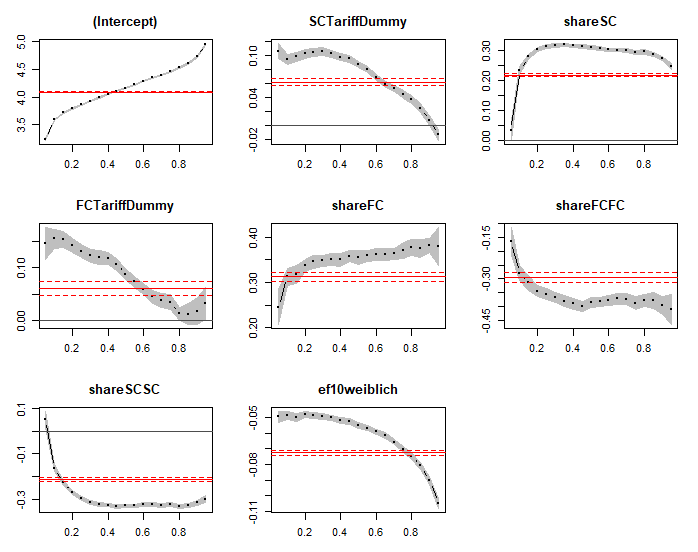
\includegraphics[width=195mm,scale=0.5]{Rplot01}\\
    \label{Fig:CQROLScomparison}
    \footnotesize Data source: GSES 2010
  \end{center}
\end{figure}
\end{landscape}
\subsection{Unconditional Quantile Regression}
\subsubsection*{Theory}
Since the conditional quantile regression approach is used to estimate the impact of a covariate on a quantile of the outcome variable, conditional on the distribution of other covariates, it lacks generalizability and the interpretation of the estimated treatment effects across quantiles becomes problematic.
Conversely, the unconditional quantile regression approach, firstly introduced by \cite{Firpo&Fortin&Lemieux:09}, marginalizes the effect over the distributions of other covariates and hence, overcomes the limitations of the conditional quantile regression approach. It is therefore advisable to use the unconditional quantile regression approach if the model contains multiple covariates and interaction effects. Unconditional quantile regressions are applicable to many research fields and have for example been used to investigate the determinants of medication adherence \citep{Borah&Basu:2013} or the effect of cigarette tax increases on smoking behavior \citep{Maclean&Marti&Webber:2014}.

There are several ways to generalize the effect of a covariate on the unconditional quantile of the outcome variable. One option is to use the coefficient estimates of the conditional quantile regression in order to recover equation \ref{4}. \cite{Firpo&Fortin&Lemieux:09} show that the unconditional quantile partial effect of a covariate $X$ on $Y$, $UQPE(\tau)$, equals a weighted average (over the distribution of $X$) of the partial effect of $X$, $CQPE(\zeta_{\tau}, X)$, on a specific conditional quantile $\zeta_{\tau}(X)$ of $Y$, corresponding to the $\tau$-th unconditional quantile of the distribution of $Y$, that we are interested in. In general, it holds true that the conditional quantile partial effect of $X$ does not average up to the effect on the same unconditional quantile, $UQPE(\tau) \neq \E[CQPE(\tau, X)]$.\footnote{ except for a linear, additively separable model} In order to gain a better understanding of the relationship between conditional and unconditional quantile partial effects let us assume that we are interested in the $UQPE$ for the median of the wage distribution, $UQPE(\tau = 0.5)$. If union coverage had a positive effect on wages, the overall median would perhaps correspond to the $25^{th}$ percentile of those covered by a union, and to the $75^{th}$ percentile of those not covered by a union: $\zeta_{0.5}(X=1)=0.25$ and $\zeta_{0.5}(X=0)=0.75$. The average of the two conditional quantile partial effects results in the unconditional quantile partial effect at the median, whereas taking the average of the medians of the two conditional quantiles may yield a different result. Hence, this approach can only be implemented if the unconditional quantiles of $Y$ can be mapped to the corresponding conditional quantiles under different conditioning arguments, which is often not feasible \citep{Borah&Basu:2013}.

The recently introduced approach by \cite{Firpo&Fortin&Lemieux:09} uses the concept of recentered influence functions (RIFs) to perform unconditional quantile regressions. The influence function is a statistical tool applicable to robust estimation of econometric models and defined as
\begin{equation}\label{8}
  IF(y;v(F))=\lim_{\epsilon \rightarrow 0}\frac{[v((1-\epsilon)F+\epsilon \delta_{y})-v(F)]}{\epsilon} , 0 \leq \epsilon \leq 1
\end{equation}
where $F$ is the sample probability distribution of $Y$ and $\delta_y$ represents the distribution for a point mass at the value $y$. Hence, the mixture distribution $(1-\epsilon)F + \epsilon \delta_{y}$ consists of the actual distribution $F$ weighted by $(1-\epsilon)$ and the value $y$ weighted by $\epsilon$. The influence function therefore assesses the marginal influence of an observation at the value $y$ on the distributional statistic $v(F)$. The recentered influence function is obtained by adding back the distributional statistic $v(F)$ to its influence function:
\begin{equation}\label{9}
  RIF(y;v)=v(F)+IF((y;v)
\end{equation}
One advantageous property of the recentered influence function is that its expectation equals the distributional statistic $v(F)$: $\E[RIF(y;v)]=v(F)$. Take for example the mean, $\mu$ as the statistic of interest, then, using L'H\^opital's rule: \footnote{ $\lim_{\epsilon \rightarrow 0}\frac{[(1-\epsilon)\mu + \epsilon y -\mu]}{\epsilon} = \frac{''0''}{''0''} \longrightarrow$ L'H\^opital's rule yields: $\frac{f'(\epsilon)}{g'(\epsilon)}=\frac{-\mu + y}{1}=y-\mu$}
\begin{equation}\label{10}
  RIF(y;\mu)=\mu + \lim_{\epsilon \rightarrow 0}\frac{[(1-\epsilon)\mu + \epsilon y -\mu]}{\epsilon}=\mu +(y-\mu)=y
\end{equation}
\begin{equation*}\label{11}
  \E[RIF(y;\mu)]=\mu
\end{equation*}
Then, the recentered influence function yields the value of Y itself, implying that regressing the recentered influence function for the mean on $X$ yields the same coefficients as an ordinary least squares regression.\\
Now, let us change the statistic of interest to a specific quantile $\tau$ of the outcome distribution and determine the influence function. Therefore, we denote the quantile of the mixture distribution as:
\begin{equation}\label{12}
  q_{\tau}((1-\epsilon)F+\epsilon \delta_{y})=q_{\tau}^{'}
\end{equation}
We have
\begin{equation*}
  (1-\epsilon)F(q_{\tau}^{'})+\epsilon \delta_{y}(q_{\tau}^{'})=\tau
\end{equation*}
with $\delta_{y}(q_{\tau}^{'})=I(Y\leq q_{\tau}^{'})$, a dummy variable determining whether the outcome variable is below $q_{\tau}$. Using the implicit function theorem leads us to:
\begin{equation*}\label{13}
  \frac{\partial q_{\tau}^{'}}{\partial \epsilon}=-\frac{-F(q_{\tau}^{'})+I(Y \leq q_{\tau}^{'})}{(1-\epsilon)f_{Y}(q_{\tau}^{'})}
\end{equation*}
For $\epsilon \rightarrow 0$, $q_{\tau}^{'} \rightarrow q_{\tau}$ and $F(q_{\tau}^{'}) \rightarrow \tau$
\begin{equation}\label{14}
  IF(y;q_{\tau})=\frac{\tau - I(Y \leq q_{\tau})}{f_{Y}(q_{\tau})}
\end{equation}
where $q_{\tau}$ represents the $\tau$-th quantile of the unconditional distribution of $Y$ and $f_{Y}(q_{\tau})$ refers to the probability density function of $Y$. Consequently, the recentered influence function is:
\begin{equation}\label{15}
  RIF(y;q_{\tau})=q_{\tau}+IF(y;q_{\tau})=q_{\tau} + \frac{\tau - I(Y \leq q_{\tau})}{f_{Y}(q_{\tau})}
\end{equation}
\cite{Firpo&Fortin&Lemieux:09} call the expectation of the $RIF(Y; v,F_{Y})$, conditional on the explanatory variables $X$, the \emph{RIF regression model}, $\E[RIF(Y; v, F_{Y})|X]=m_{v}(X)$. Constructed for quantiles, $\E[RIF(Y; q_{\tau,} F_{Y})|X]=m_{\tau}(X)$ represents an \emph{unconditional quantile regression}. Furthermore, they show that the average derivative of the unconditional quantile regression, $\E[m_{\tau}^{'}(X)]$, can be interpreted as the marginal effect on the unconditional quantile of interest, resulting from a small location shift in the distribution of covariates, ceteris paribus. Similarly to an OLS regression, the recentered influence function can be regressed on the set of covariates $X$. Therefore, we need to estimate
\begin{equation*}
  \widehat{RIF}(Y; \hat{q}_{\tau})=\hat{q}_{\tau}+ \frac{\tau - I(Y \leq \hat{q}_{\tau})}{\hat{f}_{Y}(\hat{q}_{\tau})}.
\end{equation*}
The estimated density of $Y$, $\hat{f}_{Y}(\hat{q}_{\tau})$ can be obtained by using, for example, the kernel density estimator, whereas $\hat{q}_{\tau}$ is determined by estimating the unconditional quantile $\tau$, based on the sample at hand.
\subsubsection*{Implementation}
In order to employ unconditional quantile regression, we employ the package \texttt{uqr}.
\lstset{firstnumber = 491}
\begin{lstlisting}
install.packages("uqr")
library(uqr)
\end{lstlisting}
Since our quantiles of interest are now reduced to only five, because we do not create another graphic comparison, we define a vector, which specifies the quantiles that the regression should be executed for.
\lstset{firstnumber = 494}
\begin{lstlisting}
quantile2=c(0.1, 0.25, 0.5, 0.75, 0.9)
\end{lstlisting}
Applying the \texttt{uqr} function to our model, with \texttt{lnWage} as the dependent variable and all following variables as the explanatory variables, we can estimate unconditional quantile regression coefficients. Again, we are using the data set \texttt{quantileRegressionData} and our previously defined vector of quantiles of interest. Our results are saved in \texttt{modelUnconditionalQR}.
\lstset{firstnumber = 495}
\begin{lstlisting}
modelUnconditionalQR = urq(lnWage ~  SCTariffDummy + shareSC + FCTariffDummy + shareFC + shareFCFC + shareSCSC + ef10 + east + ef9be + ef12be + ef26be + minimumWage + ef9 + educ2 + educ3 + shift + ef40 + agesq + ef41 + expsq + permanent, data=quantileRegressionData, tau = quantile2 )
\end{lstlisting}
The calculation of the unconditional average partial effects is implemented in the same way as the calculation for the conditional average partial effects, which has been described in section \ref{cqrimplement}. The results of the calculation are summarized in the table \texttt{\dq averagePartialEffectUQR.tex\dq} and put out in \LaTeX-code.
\lstset{firstnumber = 518}
\begin{lstlisting}
print(xtable(averagePartialEffectUQR, type = "latex"), file = "averagePartialEffectUQR.tex") #print table in latex code
\end{lstlisting}
In order to test coefficients for significance, we are constructing confidence intervals for the obtained coefficients, determining the standard errors and p-values, using bootstrapping with \texttt{R = 30} replications. The remaining options are set to default values.
\lstset{firstnumber = 521}
\begin{lstlisting}
modelUnconditionalQR.BCI = urqCI(modelUnconditionalQR , R = 30, seed=NULL , colour=NULL , confidence=NULL , graph=TRUE , cluster=NULL , BC=FALSE)
\end{lstlisting}
\subsubsection*{Results}
The results of the unconditional quantile regression are displayed in table \ref{UQRimplement} and the resulting unconditional average partial effects are summarized in table \ref{APEs:UQRimplement}. Similarly to the OLS regression, the coefficients of the quantile regression can now be interpreted as effects on the unconditional wage distribution.

Compared to the conditional quantile regression estimates, the coefficients obtained by an unconditional quantile regression have significantly larger spreads across the wage distribution. For example, the individual union wage premium for an employee, covered by a sectoral contract in a firm with an average coverage ratio, declined monotonically from $4\%$ at the 10th percentile to $-10\%$ at the 90th percentile in a conditional quantile regression setting. In contrast, the average partial effect for individual coverage at the sectoral level decreases from $20\%$ at the 10th percentile to $-51\%$ at the 90th percentile of the unconditional wage distribution. This means that an employee, working under a sectoral collective contract in a firm with an average coverage ratio earns on average $20\%$ more than an uncovered employee in the same firm, at the 10th percentile. At the top end of the wage distribution (90th percentile), the uncovered employee earns on average $51\%$ more than the covered employee. The reason for that trend may be that firms want to pay a premium to highly productive employees, e.g. employees with management responsibilities. Furthermore, these employees cannot rely on a collective contract as a fall back position and are therefore paid a risk premium, as argued before. For firm-level coverage the effects are estimated to be less drastic, meaning that the union wage premium for covered employees at the bottom end of the distribution is less than under a sectoral contract. In return, the negative union wage premium at the top of the distribution is lower than under sectoral bargaining coverage as well. Under firm-level coverage, effects remain fairly constant and positive over quantiles, before they drop and become negative towards the top of the distribution.
The average partial effects for an increase in the share of covered employees within a firm, under both coverage regimes, are different from the effects obtained in table \ref{APEs:CQRimplement}. While the effect is negative at lower quantiles, the effects become larger and positive at the top end of the wage distribution for both coverage regimes. For example, a $10\%$ increase in the share of covered employees by a sectoral contract in a firm with an average coverage rate, leads to a $-1.6\%$ decrease in wages at the 10th percentile and a $6.6\%$ increase at the 90th percentile of the unconditional wage distribution. Therefore, an increasing share of covered employees contributes to wage dispersion. Whereas the interaction coefficients are negative at all quantiles and only tendentially declining across quantiles in table \ref{CQRresults}, they decrease significantly more using unconditional quantile regression, and are even positive on lower quantiles. Hence, the effect of individual coverage in high coverage firms is particularly positive for employees on lower quantiles and particularly negative for employees on higher quantiles. Similarly to the conditional quantile regression results, the unconditional quantile regression results yield a significant gender wage gap. The gender wage gap increases over quantiles from $0.8\%$ at the 10th percentile to $17.7\%$ at the 90th percentile.
\begin{landscape}
\begin{table}[]
\scriptsize
\centering
\caption{Unconditional Quantile Regression Results}
\label{UQRimplement}
\begin{tabular}{l|cccccccccc}
 percentile & \multicolumn{2}{c}{(10)} & \multicolumn{2}{c}{(25)} & \multicolumn{2}{c}{(50)} & \multicolumn{2}{c}{(75)} & \multicolumn{2}{c}{(90)}\\
\hline
 & coef. & std. err. & coef. & std. err. & coef. & std. err. & coef. & std. err. & coef. & std. err. \\
\hline
Sector Contract (SC)    & $0.155^{**}$ & $(0.001)$ & $0.200^{**}$ & $(0.001)$ & $0.096^{**}$ & $(0.000)$ & $0.028^{**}$ & $(0.001)$ & $-0.175^{**}$ & $(0.001)$\\
Firm Contract (FC)      & $0.058^{**}$ & $(0.001)$ & $0.146^{**}$ & $(0.001)$ & $0.106{**}$ & $(0.000)$ & $0.174^{**}$ & $(0.001)$ & $-0.101^{**}$ & $(0.001)$\\
shareSC                 & $-0.208^{**}$ & $(0.001)$ & $0.055^{**}$ & $(0.001)$ & $0.141^{**}$ & $(0.000)$ & $0.279^{**}$ & $(0.001)$ & $0.996^{**}$ & $(0.004)$\\
shareFC                 & $-0.070^{**}$ & $(0.001)$ & $0.133^{**}$ & $(0.001)$ & $0.168^{**}$ & $(0.000)$ & $0.318^{**}$ & $(0.001)$ & $0.939^{**}$ & $(0.004)$\\
shareSCxSC              & $0.131^{**}$ & $(0.002)$ & $-0.078^{**}$ & $(0.001)$ & $-0.057^{**}$ & $(0.000)$ & $-0.283^{**}$ & $(0.001)$ & $-0.958^{**}$ & $(0.004)$\\
shareFCxFC              & $0.134^{**}$ & $(0.001)$ & $-0.015^{**}$ & $(0.001)$ & $-0.110^{**}$ & $(0.000)$ & $-0.544^{**}$ & $(0.002)$ & $-0.963^{**}$ & $(0.004)$\\
gender (male=0)         & $-0.008^{**}$ & $(0.000)$ & $-0.023^{**}$ & $(0.000)$ & $-0.029^{**}$ & $(0.000)$ & $-0.106^{**}$ & $(0.000)$  & $-0.177^{**}$ & $(0.001)$\\
\hline
$N$                     & \multicolumn{2}{c}{700886} & \multicolumn{2}{c}{700886} & \multicolumn{2}{c}{700886} & \multicolumn{2}{c}{700886} & \multicolumn{2}{c}{700886} \\
\hline
\end{tabular}\\
\bigskip
Unconditional quantile regression includes a full set of firm-specific and individual-worker covariates.\\
$^{*}$/$^{**}$: significance at the 5\%/1\% -level
\end{table}
\begin{table}[]
\scriptsize
\centering
\caption{Average Partial Effects obtained by Unconditional Quantile Regression}\vspace{0.2cm}
\label{APEs:UQRimplement}
\begin{tabular}{rlrrrrr}
  \hline
 & Quantiles & tau10 & tau25 & tau50 & tau75 & tau90 \\
  \hline
1 & Sector Contract (SC) & 0.20 & 0.17 & 0.08 & -0.07 & -0.51 \\
  2 & shareSC & -0.16 & 0.03 & 0.12 & 0.18 & 0.66 \\
  3 & Firm Contract (FC) & 0.07 & 0.14 & 0.10 & 0.14 & -0.16 \\
  4 & shareFC & -0.06 & 0.13 & 0.16 & 0.29 & 0.88 \\
   \hline
\end{tabular}
\end{table}
\end{landscape}



\section{Conclusions}\label{Sec:Conc}
In this paper, we analyze the effect of collective bargaining coverage on wages and its implications for wage dispersion in Germany. Our analysis distinguishes between individual coverage on the sectoral level and firm-level and the within-firm coverage ratios for both bargaining regimes. The econometric investigation is conducted using a linked employer-employee dataset, the German Structure of Earnings Survey 2010, provided by the Research Data Centers of the Federal Statistical Office and the statistical offices of the L\"ander. Throughout my analysis we control for individual and firm characteristics in order to reduce the endogeneity problem of collective coverage, i.e. the selection bias based on observable characteristics, but of course, we cannot rule out selection on unobservable characteristics. For example, there might be a selection bias with regard to the productivity distribution in the covered and uncovered sector since the more productive workers should have a preference for the uncovered sector according to the \emph{worker-choice model} \citep{Lee:78}. An alternative selection bias might occur when employers hire more highly productive employees in response to the presence of a union, adapting to the high wages of less-qualified workers. Combining the two examples yields that the unionized sector is mainly composed of employees with an average productivity. Highly productive workers refuse to be unionized and low productive workers will not be hired. Additionally, the assumption of an exogenous coverage ratio could be violated if workers especially try to organize in industries with potentially high gains from unionization. 

Using OLS regression as well as conditional and unconditional quantile regressions, we come to the following conclusions. The share of covered employees within a firm has a positive effect on wages and increases along the unconditional wage distribution. Thus, firms that apply a collectively negotiated contract pay higher wages than uncovered firms, particularly benefitting high-wage earners. This finding suggests that a higher share of covered employees within a firm contributes to wage dispersion. \cite{Fitzenberger&Kohn&Lembcke:13} confirm the positive effect on wages, but find a fairly constant impact across conditional quantiles of the wage distribution. Our conditional quantile regression results are in line with the estimates obtained by \cite{Fitzenberger&Kohn&Lembcke:13}. Holding the coverage share in the firm constant, individual coverage under sectoral and firm-level contracts show a positive effect for lower quantiles, which turns negative towards the top of the unconditional wage distribution. Thus, individual coverage by any of the two coverage regimes reduces wage dispersion.

Since wage inequality in many industrialized countries, including Germany, has risen over the last couple of decades and union density as well as collective bargaining coverage declined over the same period, future research should further investigate the causal relationship between the two developments, based on \cite{Antonczyk&&&:11} and \cite{Dustmann&Ludsteck&Schönberg:09}.



%making sure that all sources are cited


% ----------------
% --- appendix ---
% ----------------
\appendix

% literature
\newpage
\renewcommand{\thepage}{\roman{page}} \setcounter{page}{4}
\addcontentsline{toc}{section}{References}
\bibliography{literature}

\newpage
\section{Tables}

\begin{table}[H]
\centering
\caption{Part 1: Overview of the raw data}
\label{raw1}
\begin{tabular}{|l|l|l|l|}
\hline
\textbf{Variable} & \textbf{Label}                                               & \textbf{Min}  & \textbf{Max}    \\ \hline
ef1      & ID-number of the firm                               & 1    & 32219  \\ \hline
ef2      & Type of questionnaire                               & 1    & 1      \\ \hline
ef3      & Consecutive number of the worker in the firm        & 1    & 4214   \\ \hline
ef8      & Type of union contract                              & 0    & 2      \\ \hline
ef9      & Performance group for compensation                  & 1    & 5      \\ \hline
ef10     & Gender                                              & 1    & 2      \\ \hline
ef15     & Profession                                          & 10   & 71     \\ \hline
ef16u1   & Positio in the profession                           & 0    & 9      \\ \hline
ef16u2   & Education                                           & 1    & 7      \\ \hline
ef17     & Type of contract                                    & 1    & 5      \\ \hline
ef18     & Regular working time                                & 0    & 80     \\ \hline
ef19     & Paid working hours without overtime                 & 0,44 & 347,6  \\ \hline
ef20     & Paid overtime                                       & 0    & 311,5  \\ \hline
ef21     & Total gross monthly income                          & 1    & 163035 \\ \hline
ef22     & Total income for overtime                           & 0    & 12015  \\ \hline
ef23     & Bonuses for layering work/ night work/ …            & 0    & 6137   \\ \hline
ef24     & Income tax                                          & 0    & 70237  \\ \hline
ef25     & Total social security contributions                 & 0    & 1502   \\ \hline
ef26     & Social insurance workdays during the reporting year & 0    & 360    \\ \hline
ef27     & Total (year) gross income                           & 10   & 750000 \\ \hline
ef28     & Special payments                                    & 0    & 577500 \\ \hline
ef29     & Holiday entitlement                                 & 0    & 99     \\ \hline
ef36     & Basis of holiday calculation                        & 4    & 7      \\ \hline
ef38     & Grossing-up factor for employees                    & 0,49 & 521,93 \\ \hline
ef40     & Work experience                                     & 0    & 45     \\ \hline
\end{tabular}
\end{table}

\begin{table}[H]
\centering
\caption{Part 2: Overview of the raw data}
\label{raw2}
\begin{tabular}{|l|l|l|l|}
\hline
\textbf{Variable} & \textbf{Label}                                               & \textbf{Min}  & \textbf{Max}    \\ \hline
ef41     & Age                                                 & 16   & 66     \\ \hline
ef42       & Profession according to ISCO                           & 11     & 99      \\ \hline
ef43       & Education according to ISCED                           & 2      & 5       \\ \hline
ef44       & Monthly net income                                     & 1      & 93150   \\ \hline
ef48       & Monthly gross income                                   & 0,11   & 936,98  \\ \hline
ef49       & Converted holidays                                     & 0      & 99      \\ \hline
ef50       & Number of working weeks                                & 4,35   & 52,14   \\ \hline
ef51       & Paid working hours                                     & 0      & 1       \\ \hline
ef52       & Proportionate working hours of a part-time employee    & 0,25   & 100     \\ \hline
ef2be      & Type of questionnaire                                  & 0      & 0       \\ \hline
ef4be      & Regional basis                                         & 1      & 6       \\ \hline
ef6be      & Industry                                               & 5      & 95      \\ \hline
ef9be      & Involvement of public in the company's capital & 1      & 2       \\ \hline
ef10be     & Employees of the company                               & 1      & 3       \\ \hline
ef11be     & Share of male workers in the firm                      & 0      & 100     \\ \hline
ef12be     & Share of female workers in the firm                    & 0      & 100     \\ \hline
ef14be     & Basis of holiday calculation                           & 4      & 7       \\ \hline
ef15be     & Normal weekly work time                                & 30     & 63,69   \\ \hline
ef16abe    & Collective agreement                                   & 0      & 1       \\ \hline
ef16bbe    & Type of collective agreement                           & 0      & 2       \\ \hline
ef21be     & Grossing-up factor level 1                             & 0,3643 & 207     \\ \hline
ef22be     & Grossing-up factor level 2                             & 1      & 274,831 \\ \hline
ef23be     & Addition coefficient                                   & 1      & 3       \\ \hline
ef26be     & Number of the employees of the enterprise                            & 1      & 44523   \\ \hline
ef26be\_ma & Number of the employees of the enterprise microaggregated           & 1      & 2       \\ \hline
ef31be     & Minimum wage industries                                & 1      & 3       \\ \hline
\_merge    & Merge factor                                           & 3      & 3       \\ \hline
\end{tabular}
\end{table}
\newpage
\section{Figures}

\begin{figure}[H]
  \begin{center}
   \caption{Trade Union Density and Collective Bargaining Coverage, 1990 and latest year}
   \bigskip
    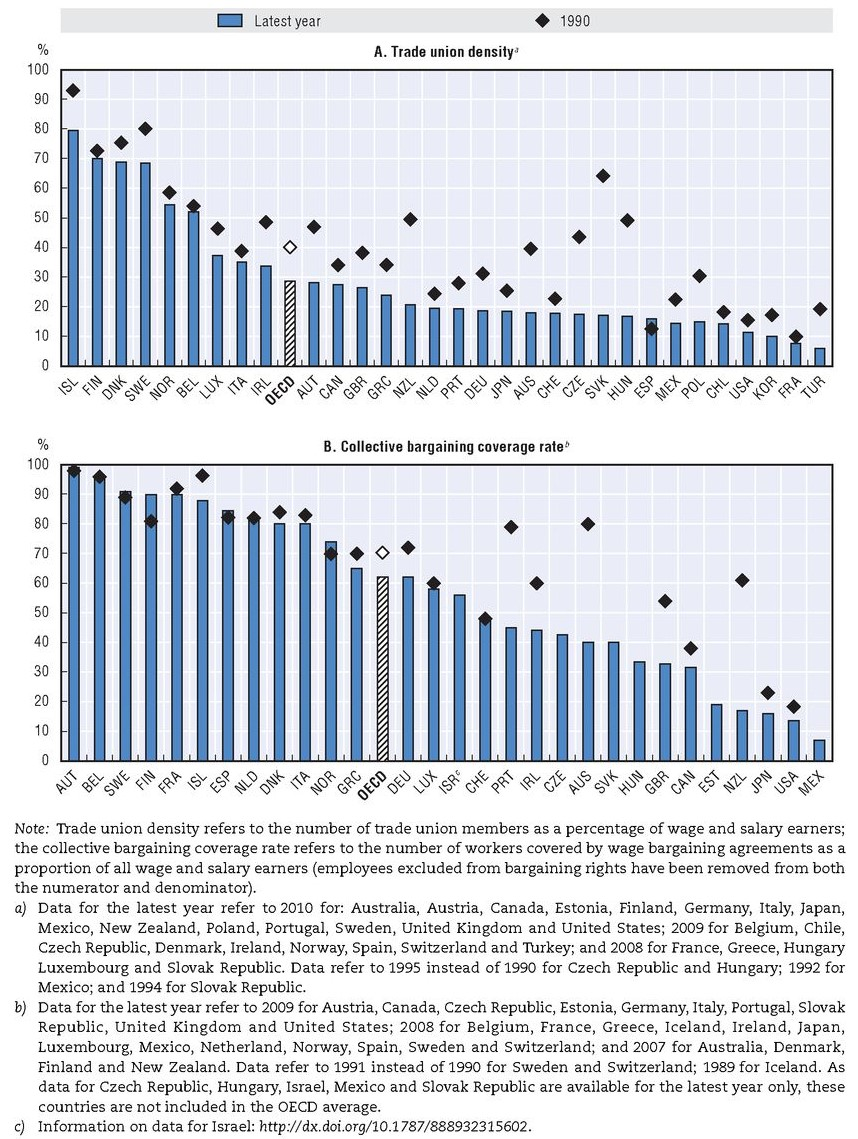
\includegraphics[width=135mm,scale=0.5]{UDandCC2}\\
    \label{Fig:UDandCC2}
    \footnotesize Source: \cite[p.~136]{OECD:12}
  \end{center}
\end{figure}

\begin{figure}[H]
  \begin{center}
   \caption{Boxplot of education differences in ln(Wage) of the population with union contract}
    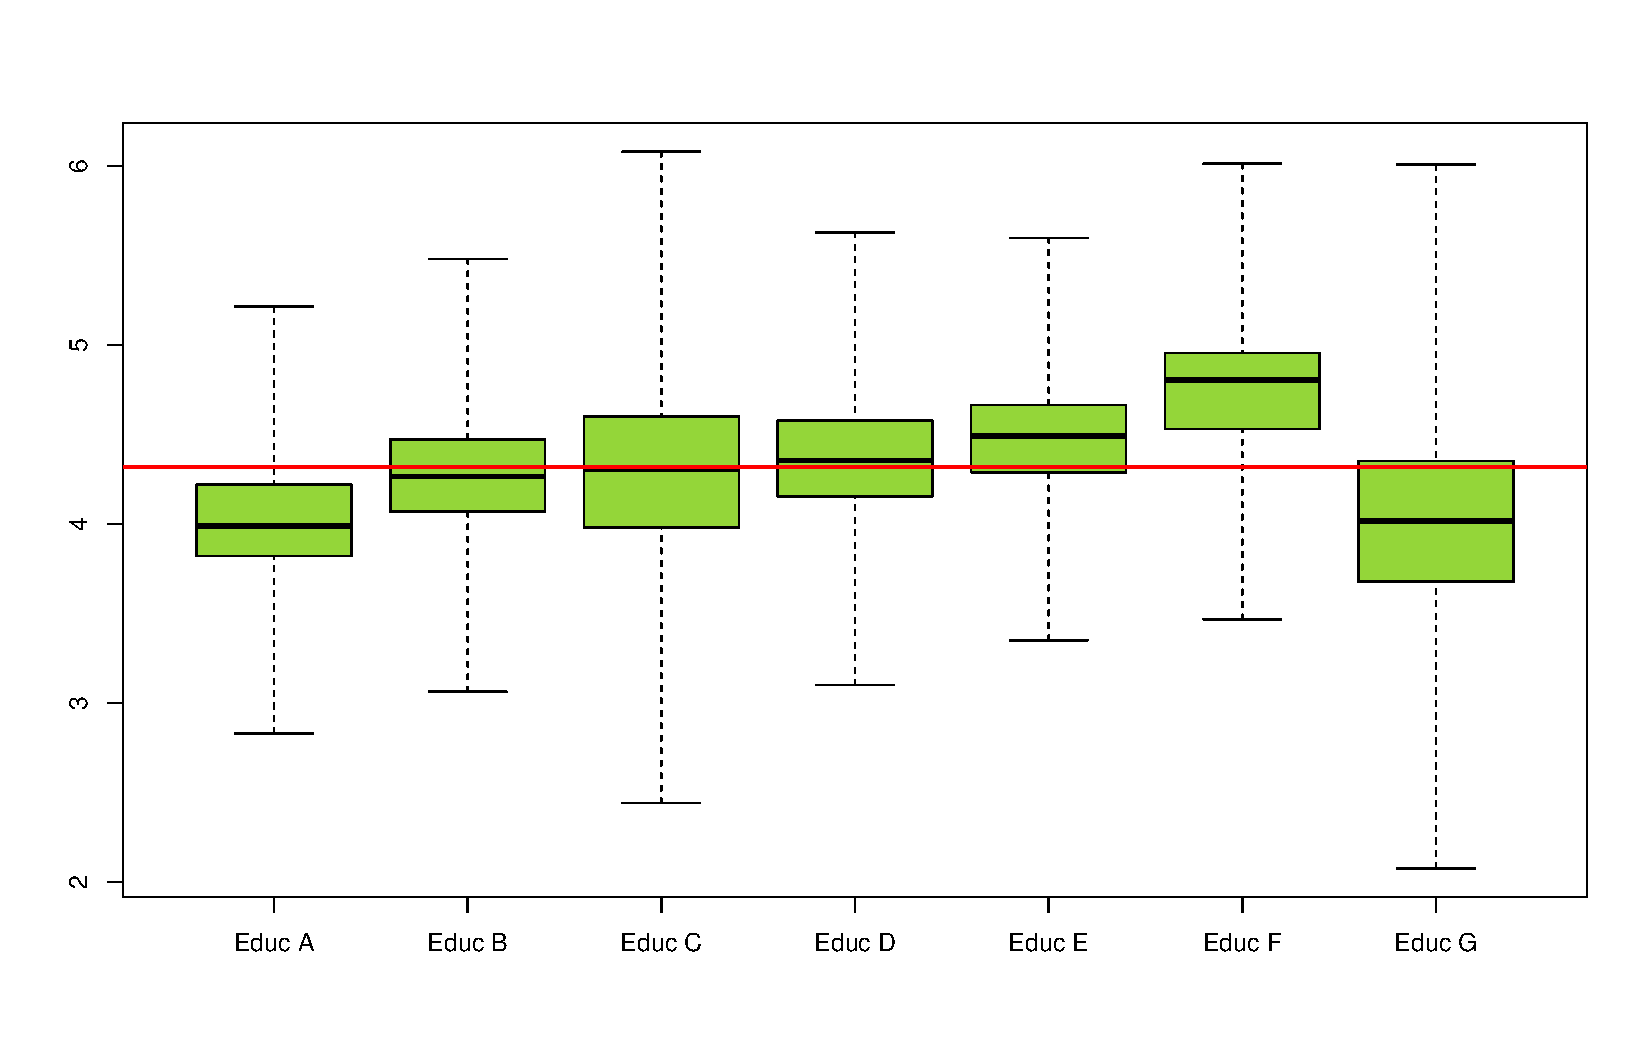
\includegraphics[scale=0.5]{boxploteducFCSC}\\
    \label{Fig:educFCSC}
  \end{center}
\end{figure}

\begin{figure}[H]
  \begin{center}
   \caption{Boxplot of education differences in ln(Wage) of population without union contract}
    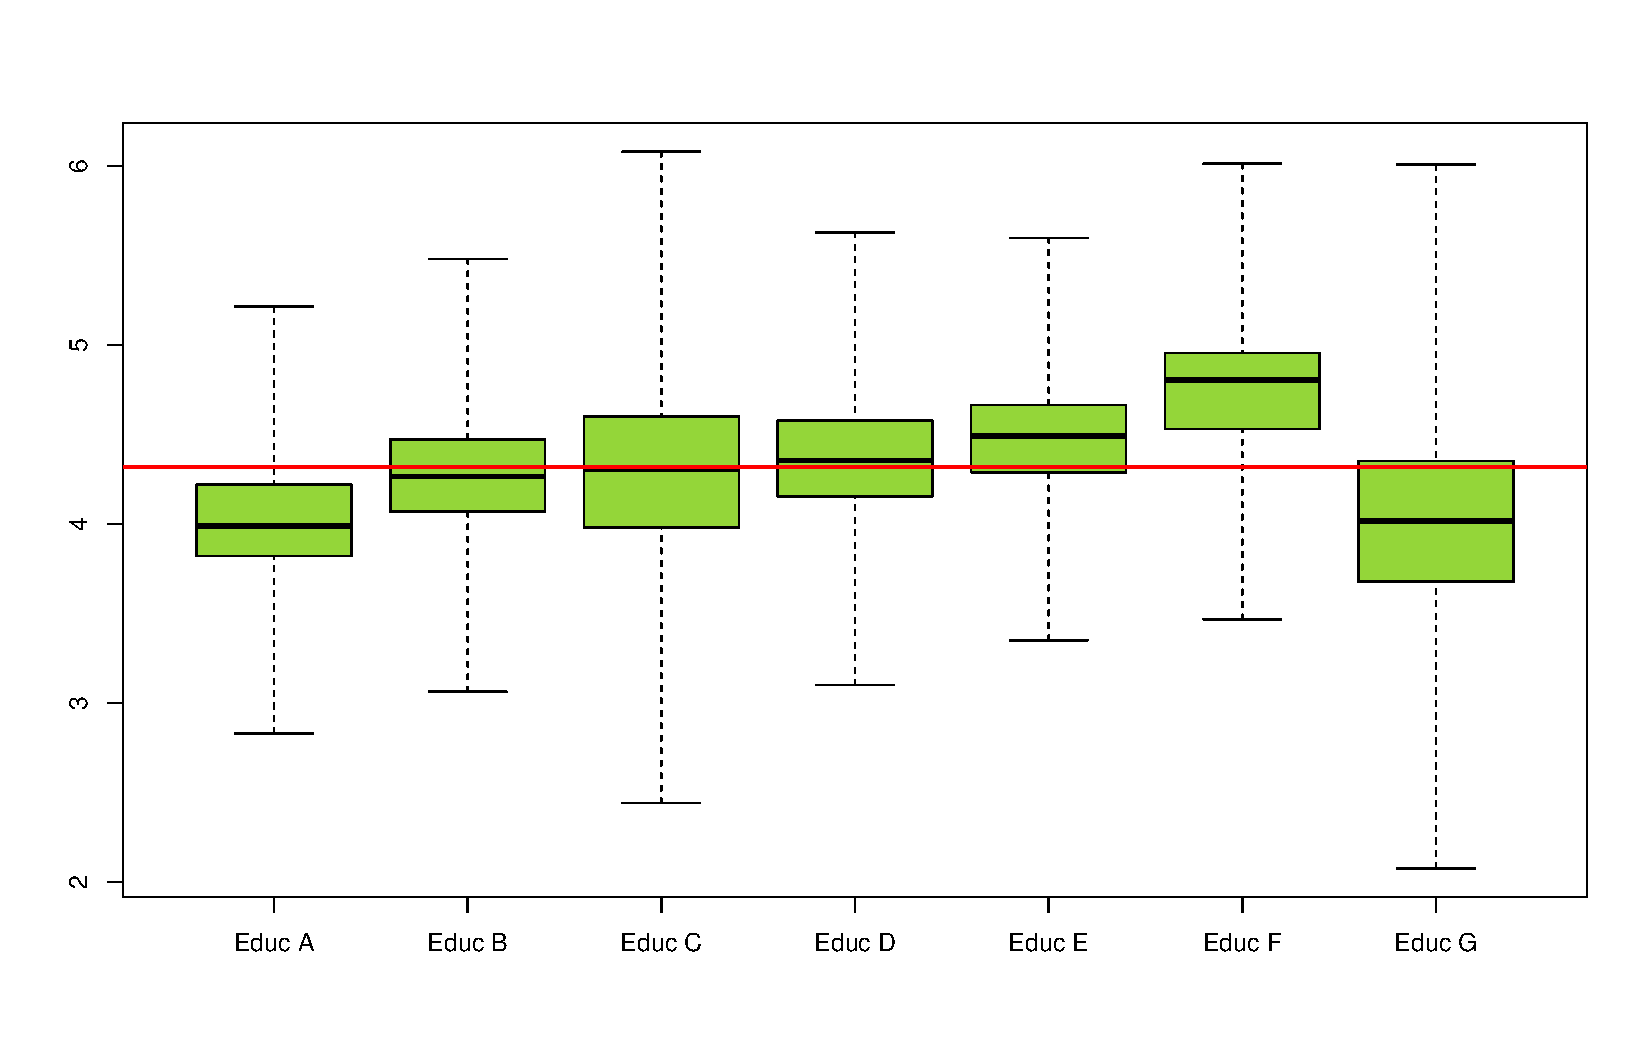
\includegraphics[scale=0.5]{boxploteducFCSC}\\
    \label{Fig:educNoFCSC}
  \end{center}
\end{figure}
\newpage
\section{Code}

Please note that the quantlets are all related to their order and are specifically adapted to the data set \texttt{dataset2010.dta}. The quantlets must be executed in their order to obtain the same results as presented in this paper.


\subsection{Code for Data Preparation}

\subsubsection{Code for Quantlet 1}
\lstset{firstnumber = 1}
\begin{lstlisting}
#clear the workspace
rm(list=ls())

#install package / load library for importing stata 13 files
install.packages("readstata13")
library(readstata13)

#importing the data into dat
dat = read.dta13("dataset2010.dta", convert.factors = TRUE, 
	generate.factors = FALSE, encoding = "UTF-8",  fromEncoding = NULL,  
	convert.underscore = FALSE, missing.type = FALSE, convert.dates = TRUE, 
	replace.strl = TRUE, add.rownames = FALSE, nonint.factors = FALSE,
	select.rows = NULL)

#function for calculation respondents per company
respondFunc = function(dat){
  if (missing(dat)) 		stop("No data passed to the function")
  if (is.numeric(dat)!= TRUE)	stop("Numeric data needed")
  respond = numeric(length(dat))
  i = 1                                   #setting counting variables to 1
  j = 1
  temp = table(dat)                       #how many different values are in dat
  for (i in 1:length(dat)){               #for every observation
    j = dat[i]                            #store value of dat in j
    respond[i] = temp[j]                  #value of temp[i] store in respond[i]
    i = i+1              
  }
  return(respond)
}

respond = respondFunc(dat$ef1)			#call function respondFunc
dat["respond"] = respond			#add to data frame

#dummyfunction to create dummy variables,
#compare data vector with selected level of data vector, 
#if true, then function writes 1
dummyFunc = function(dat , x){
  if (missing(dat))			stop("No data passed to the function")
  if(is.null(levels(dat)))		stop("No levels found")
  d = as.numeric(dat == levels(dat)[x])      
  return(d)
}

#create eastdummy  0=west
east = dummyFunc(dat$ef4be , 5)  		#call function dummyFunc
dat["east"] = east           	    		#add to data frame

#create less classes for education
tempEdu1  = dummyFunc(dat$ef16u2 , 1 )
tempEdu1a = dummyFunc(dat$ef16u2 , 2 )
tempEdu2  = dummyFunc(dat$ef16u2 , 3 )
tempEdu2a = dummyFunc(dat$ef16u2 , 4 )
tempEdu3  = dummyFunc(dat$ef16u2 , 5 )
tempEdu3a = dummyFunc(dat$ef16u2 , 6 )
tempNa    = dummyFunc(dat$ef16u2 , 7 )
tempNa[tempNa == 1] = NA               		 #add NA's from dataset

#reduce dummy levels from 6 to 3
educ1 = tempEdu1 + tempEdu1a + tempNa   
educ2 = tempEdu2 + tempEdu2a + tempNa
educ3 = tempEdu3 + tempEdu3a + tempNa

dat["educ1"] = educ1                  	 	#add to data frame
dat["educ2"] = educ2
dat["educ3"] = educ3

#create dummy for permanent workers
permanent        = dummyFunc(dat$ef17 , 1 )
dat["permanent"] = permanent        		 #add to data frame

#define whether someone worked in shifts/at night/...
shift        = as.numeric(dat$ef23 >= 1)
dat["shift"] = shift                   		 #add to data frame

#create dummy for fulltime workers and reduce levels 
tempFull1 = as.numeric(dat$ef16u1 != "Teilzeitbeschäftigt - Beamter")
tempFull2 = as.numeric(dat$ef16u1 != "Teilzeitbeschäftigt - weniger als 18 Std.")
tempFull3 = as.numeric(dat$ef16u1 != "Teilzeitbeschäftigt - 18 Std. und mehr")
fulltime  = tempFull1+tempFull2+tempFull3 - 2
dat["fulltime"] = fulltime        		   #add to data frame

#create minimumwage dummy 0=nein 
minimumWage   = as.numeric(dat$ef31be != "nein")
minimumWageNa = dummyFunc(dat$ef31be , 3 )
minimumWageNa[minimumWageNa == 1] = NA 	 		#add NA's from dataset
minimumWage        = minimumWage+minimumWageNa
dat["minimumWage"] = minimumWage + minimumWageNa       #add to data frame
\end{lstlisting}


\subsubsection{Code for Quantlet 2}
\lstset{firstnumber = 89}
\begin{lstlisting}
#create function to calculate how many employees have a union contract or not
#a= company dummy, b= data information vector with dummies, c= choose level
contractFunc = function(a,b,c){            
  if (missing(b)) 		stop("No data passed to the function")
  if (is.numeric(a)!= TRUE & is.numeric(b)!= TRUE  )
    stop("numeric data needed")
  if (missing(c))		stop("No level selected")
  temp = table(a)
  #calculate cummulative sums for later addressing the vector
  cumtemp = cumsum(temp)                 
  cumtemp = append(cumtemp,0,after =0)     #need 0 as start value 
  g = nrow(temp) +1
  i = 2                                    #setting counting variables to 1
  j = 1
  k = 1
  q = numeric(length(b))
  for (i in 2:g){
    k = cumtemp[i-1]+1                   #store starting value company x in dat in k
    j = cumtemp[i]                       #store end value company x in dat in j
    #store results in p (how many people have kein Tarifvertrag and so on....)
    p = table(b[k:j])                      
    q[k:j]  = p[c]                   
    i = i+1
  }
  return(q)
}

noTariff = contractFunc(dat$ef1, dat$ef8, 1) 	#call function contractFunc
SCTariff = contractFunc(dat$ef1, dat$ef8, 2)
FCTariff = contractFunc(dat$ef1, dat$ef8, 3)
dat["noTariff"] = noTariff               	 #add to data frame
dat["SCTariff"] = SCTariff
dat["FCTariff"] = FCTariff

#create shares
shareFC = FCTariff/respond
shareSC = SCTariff/respond
dat["shareFC"] = shareFC           		 #add to data frame
dat["shareSC"] = shareSC

#create dummy variables for no labor, sectoral and firm-level contract
noTariffDummy = dummyFunc(dat$ef8 , 1)
SCTariffDummy = dummyFunc(dat$ef8 , 2)
FCTariffDummy = dummyFunc(dat$ef8 , 3)
dat["noTariffDummy"] = noTariffDummy          	#add to data frame
dat["SCTariffDummy"] = SCTariffDummy
dat["FCTariffDummy"] = FCTariffDummy

#create interaction terms
shareFCFC = shareFC*FCTariffDummy
shareSCSC = shareSC*SCTariffDummy
dat["shareFCFC"] = shareFCFC          		#add to data frame
dat["shareSCSC"] = shareSCSC

#create variables age squared and experienece squared 
agesq = dat$ef40*dat$ef40
expsq = dat$ef41*dat$ef41
dat["agesq"] = agesq         			#add to data frame
dat["expsq"] = expsq

#define wage and lnwage
wage   = ifelse(dat$ef18+dat$ef20 == 0, NA, 
	(dat$ef21+dat$ef22)/(dat$ef18+dat$ef20))
lnWage = log(wage)
dat["wage"]   = wage              		#add to data frame
dat["lnWage"] = lnWage
\end{lstlisting}

\subsection{Code for Descriptive Analysis}
\subsubsection{Code for Quantlet 3}
\lstset{firstnumber = 156}
\begin{lstlisting}
#install and load plotrix-package / neccessary to use pyramid.plot
install.packages("plotrix")
library("plotrix")

#function to calculate relative frequencies in % table for variable k with l different characteristics
frequency = function(k, l){            
  if (missing(k))
    stop("No data passed to the function. Variable k has to be defined.")
  if (missing(l))
    stop("No data passed to the function. Variable l has to be defined.")
  100*sweep(table(k,l), 2, colSums(table(k,l)), "/")
}  

#function to build population pyramid and store it as pdf
buildpopulation = function(k, l, popname){
  if (missing(popname))
    stop('No data passed to the function. Variable popname has to be defined.
         Please define a plot name such as "populationpyramid.pdf". 
         Use quotation marks, at the beginning and the end of the plot name.')
  pop = frequency(k, l)
  pdf(popname)
  pyramid.plot(pop[,1], pop[,2], labels = rownames(pop), gap = 2,
               lxcol = "blue", rxcol = "red")
  dev.off() 
}

#subsample with employees covered by the union contract (with FC or SC)
datFCSC = dat[ which(SCTariffDummy == 1 | FCTariffDummy == 1),]

#subsample with employees not covered by the union contract (no FC & no SC)
datNoFCSC = dat[ which(SCTariffDummy == 0 & FCTariffDummy == 0),]

#population pyramid on the whole dataset
buildpopulation(dat$ef41, dat$ef10, "population_all.pdf")

#population pyramid of employees covered by the union contract
buildpopulation(datFCSC$ef41, datFCSC$ef10, "populationFCSC.pdf")

#population pyramid of employees not covered by the union contract
buildpopulation(datNoFCSC$ef41, datNoFCSC$ef10, "population-noFCSC.pdf")

#calculate arithmetic mean
mean(dat$ef41, na.rm = TRUE)          #all population
mean(datFCSC$ef41, na.rm = TRUE)      #subsample - union covered workers
mean(datNoFCSC$ef41, na.rm = TRUE)    #subsample - workers without a union contract

#calculate median
median(dat$ef41, na.rm = TRUE)          #all population
median(datFCSC$ef41, na.rm = TRUE)      #subsample - union covered workers
median(datNoFCSC$ef41, na.rm = TRUE)    #subsample - workers without a union contract

#function to simultaneously generate and save boxplot in a pdf-file
buildboxplot =  function (v, w , boxname, z){
  if (missing(v))
    stop("No data passed to the function. Variable v has to be defined.")
  if (missing(w))
    stop("No data passed to the function. Variable w has to be defined.")
  if (missing(z))
    stop("No data passed to the function. Variable z has to be defined.
         z is a vector which should contain labels for the characteristics of 
         the variable w. The number of the characteristics of w must equal the 
         number of elements in z.")
  if (missing(boxname))
    stop('No data passed to the function.boxname has to be defined such as 
    	"graph.pdf".') 
  if (is.numeric(v)!= TRUE)
    stop("Numeric data needed. k has to be a numeric variable.")
  pdf(boxname, width = 11, height = 7)
  boxplot(v~w, range=2.5, width=NULL, notch=FALSE,varwidth=FALSE, names = z,
          boxwex=0.8, outline=FALSE, staplewex=0.5, horizontal=FALSE, 
          border="black", col="#94d639", add=FALSE, at=NULL)          
  abline(h = median(v, na.rm = TRUE), col="red", lwd = 1.5)
  dev.off()
}

#define a vector with label names for gender and education
genderLAB = c("male", "female")
educLAB = c("Educ A", "Educ B", "Educ C", "Educ D", "Educ E", "Educ F", 
		"Educ G")

#boxplot ln(wage)~gender of all employees
buildboxplot(dat$lnWage, dat$ef10, "boxplot_lnwage_gen.pdf", genderLAB)

#boxplot ln(wage)~education (educ) of all employees 
buildboxplot(dat$lnWage, dat$ef16u2, "boxplot_lnwage_educ.pdf", educLAB)

#boxplot ln(wage)~educ of employees which are covered by an union contract 
buildboxplot(datFCSC$lnWage, datFCSC$ef16u2, "boxploteducFCSC.pdf", educLAB)

#boxplot ln(wage)~educ of employees which are not covered by an union contract
buildboxplot(datNoFCSC$lnWage, datNoFCSC$ef16u2, 
	"boxploteduc-NoFCSC.pdf", educLAB)

#calculate median of the variable ln(wage)
median(dat$lnWage, na.rm = TRUE)
median(datFCSC$lnWage, na.rm = TRUE)
median(datNoFCSC$lnWage, na.rm = TRUE)
\end{lstlisting}

\subsubsection{Code for Quantlet 4}
\lstset{firstnumber = 254}
\begin{lstlisting}
#function to calculate quantiles
quant = function(y, x, q){
  if (missing(x))
    stop("No data passed to the function. Variable x has to be defined.")
  if (missing(y))
    stop("No data passed to the function. Variable y has to be defined.")
  if (missing(q))
    stop("No data passed to the function. Variable q has to be defined.")
  if (is.numeric(y)!= TRUE)
    stop("Numeric data needed. y has to be a numeric.")
  if (is.numeric(q)!= TRUE)
    stop("Numeric data needed. Quantile q was wrong specified, 
    	q can be either a value or a numeric value.")
  aggregate(y, list(x), na.rm=TRUE, quantile, q)
}

#define a vector with quantiles
q = c(0.10, 0.25, 0.50, 0.75, 0.90) 

#define a vector with used colors
color = c("orange", "red", "green", "blue", "black")

#Function to construct scatterplot with quantile lines
buildquantileplot = function(x, y, xla, yla, plotname){
  if (missing(xla))
    stop("No data passed to the function. Variable xla has to be defined.
         This is a label for the x-axis.")
  if (missing(yla))
    stop("No data passed to the function. Variable yla has to be defined.
         This is a label for the y-axis.")
  if (missing(plotname))
    stop('No data passed to the function.
    	plotname has to be defined such as "graph.pdf".') 
  pdf(plotname)
  #plot points
  plot(x, y, ylim=c(2,8), pch = 1, col="dark green", 
       xlab = xla, ylab = yla)
  #plot quantilelines
  for (l in 1:length(q)){
    lines(quant(y, x, q[l]), col = color[l], lwd =2)
  }
  dev.off()
}

#Scatterplot with quantile-lines ln(wage)~age
buildquantileplot(dat$ef41, dat$lnWage, "Age", "Ln(wage)", 
	"scatterplot_lnwage_age.pdf")

#Scatterplot with quantile-lines ln(wage)~experience
buildquantileplot(dat$ef40, dat$lnWage, "Experience", "Ln(wage)", 
	"scatterplot_lnwage_experience.pdf")

#Scatterplot with quantile-lines ln(wage)~experience
buildquantileplot(datFCSC$ef40, datFCSC$lnWage, "Experience", "Ln(wage)",
	"scatterplotFCSC_lnwage_experience.pdf")

#Scatterplot with quantile-lines ln(wage)~experience
buildquantileplot(datNoFCSC$ef40, datNoFCSC$lnWage, "Experience", "Ln(wage)",
	"scatterplotNoFCSC_lnwage_experience.pdf")

\end{lstlisting}

\subsubsection{Code for Quantlet 5}
\lstset{firstnumber = 314}
\begin{lstlisting}
#install and load data.table-package 
install.packages("data.table")    
library(data.table)   

#convert data frame into data table       
dat = data.table(dat)             		

#create group with 3 factors
dat[SCTariffDummy == 1, Group := factor(1)]   
dat[FCTariffDummy == 1, Group := factor(2)]
dat[noTariffDummy == 1, Group := factor(3)]

#name each factor
dat[, Group := factor(Group, labels = c("SC", "FC", "IC"))]	

#how many observations in total are in the data table (without nas)
sum = dat[!is.na(Group), .N]                       

#calculate mean and standard deviation of lnwage for each group and each gender
lnWageSummary = dat[!is.na(Group), .(LogHourlyWageMean = mean(lnWage, na.rm = T),
	LogHourlyWageSD = sd(lnWage, na.rm = T)), by = .(ef10, Group)]  

#order variables according to gender and group
lnWageSummary = lnWageSummary[order(ef10, Group)]               

#calculate total mean (no discrimination between gender)                     
lnWageSummaryOverall = dat[!is.na(Group), .(LogHourlyWageMean = mean(lnWage, na.rm = T),
	LogHourlyWageSD = sd(lnWage, na.rm = T)), by = .(Group)]

#order variables according to group
lnWageSummaryOverall = lnWageSummaryOverall[order(Group)]

#calculate frequencys for every group and by gender
mtable = table(dat$Group, dat$ef10)                                            

#calculate employee share (no discrimination between gender)
TotalEmpolyeeShare = dat[!is.na(Group), .(Share = .N/sum), by = .(Group)] 

#order values    
TotalEmpolyeeShare = TotalEmpolyeeShare[order(Group)]                          

#create full table with before calculcated values 
lnWageSummaryTotal = data.frame(Regime = c("SC", "FC", "IC"),
		#calculate proportion for employee share (male)                                       
	MaleEmpolyeeShare = prop.table(mtable, 2)[, 1], 
		#put male wage mean value 
	MaleLogHourlyWageMean = lnWageSummary[ef10 == "männlich", LogHourlyWageMean], 
		#put male standard deviation   
	MaleLogHourlyWageSD = lnWageSummary[ef10 == "männlich", LogHourlyWageSD], 
		#calculate proportion for employee share (female)     
	FemaleEmpolyeeShare = prop.table(mtable, 2)[, 2],  
		#put male wage mean value                            
	FemaleLogHourlyWageMean = lnWageSummary[ef10 == "weiblich", LogHourlyWageMean],
		#put male standard deviation    
	FemaleLogHourlyWageSD = lnWageSummary[ef10 == "weiblich", LogHourlyWageSD],
		#put TotalEmployee share here      
	TotalEmpolyeeShare = TotalEmpolyeeShare$Share,           
		#put Total mean wage here                     
	TotalLogHourlyWageMean = lnWageSummaryOverall$LogHourlyWageMean, 
		#put total standard deviation here                 
	TotalLogHourlyWageSD = lnWageSummaryOverall$LogHourlyWageSD,                   
	stringsAsFactors = FALSE)

#calculate Total line of before created variables 
Total = c("Total",     
		#sum over male shares (=1)   
	sum(lnWageSummaryTotal$MaleEmpolyeeShare),
		#build total of mean log wage male                              
	dat[!is.na(Group) & ef10 == "männlich", mean(lnWage, na.rm = T)], 
		#build total of standard deviation male      
	dat[!is.na(Group) & ef10 == "männlich", sd(lnWage, na.rm = T)],
		#sum over female shares (=1)      
	sum(lnWageSummaryTotal$FemaleEmpolyeeShare),                          
		#build total of mean log wage female
	dat[!is.na(Group) & ef10 == "weiblich", mean(lnWage, na.rm = T)],     
		#build total of standard deviation female
	dat[ef10 == "weiblich", sd(lnWage, na.rm = T)],
		#sum over all shares (=1 , no discromination in gender)	                         
	sum(lnWageSummaryTotal$TotalEmpolyeeShare),                             
		#build total of mean log wage of all observations
	dat[!is.na(Group), mean(lnWage, na.rm = T)],                            
		#build total of standard deviation of all observations
	dat[!is.na(Group), sd(lnWage, na.rm = T)])                              

#combine total table and summary table
lnWageSummaryTotal = rbind(lnWageSummaryTotal, Total)  
 
lnWageSummaryTotal[,2:10] = rapply(lnWageSummaryTotal[,2:10], as.numeric)
lnWageSummaryTotal = rapply(object = lnWageSummaryTotal, f = round, 
	classes = "numeric", how = "replace", digits = 2)	#round results

dat = data.frame(dat)   #put data back into data frame

#install and load xtable-package
install.packages("xtable")
library(xtable)

#print file with latex code
print(xtable(lnWageSummaryTotal, type = "latex"), 
	file = "covRegimeandLNWages.tex") 

\end{lstlisting}

\subsection{Code for Regression Analysis}
\subsubsection{Code for Quantlet 6}
\lstset{firstnumber = 415}
\begin{lstlisting}
#install and load dplyr- and stargazer-package
install.packages("dplyr")
library(dplyr)
install.packages("stargazer")
library(stargazer)

#OLS regression with 4 different specifications
model1 = lm (lnWage ~ SCTariffDummy + FCTariffDummy  + ef10 + east + ef9be + ef12be + ef26be + minimumWage + ef9 + educ2 + educ3 + shift + ef40 + agesq + ef41 + expsq + permanent , dat)

model2 = lm (lnWage ~ shareSC + shareFC + ef10 + east + ef9be + ef12be + ef26be + minimumWage + ef9 + educ2 + educ3 + shift + ef40 + agesq + ef41 + expsq + permanent , dat)

model3 = lm (lnWage ~ SCTariffDummy + shareSC + FCTariffDummy + shareFC + ef10 + east + ef9be + ef12be + ef26be + minimumWage + ef9 + educ2 + educ3 + shift + ef40 + agesq + ef41 + expsq + permanent , dat)

model4 = lm (lnWage ~ SCTariffDummy + shareSC + FCTariffDummy + shareFC + shareSCSC + shareFCFC + ef10 + east + ef9be + ef12be + ef26be + minimumWage + ef9 + educ2 + educ3 + shift + ef40 + agesq + ef41 + expsq + permanent , dat)

#output table result in latex code
stargazer(model1, model2, model3, model4, title="Results OLS Regression" ,
	keep = c("SCTariffDummy", "FCTariffDummy", "shareSC" , "shareFC" , "shareSCSC" , "shareFCFC" , "ef10") , 
	covariate.labels=c("Sectoral Contract","Firm Contract", "share SC","share FC","shareSCxSC","shareFCxFC" , "gender (male = 0)"),
	align=TRUE , omit.stat=c("ser","f"),  no.space=TRUE, out = "olsregression.tex")

### Quantile Regression ###

#install and load quantreg-package
install.packages("quantreg")
library(quantreg)

#free up additional memory
memory.limit(10000)   

#delete NAs from lnwage
quantileRegressionData   = dat %>% filter(!is.na(lnWage)) 

#set quantiles
quantile = seq(0.05, 0.95, by=0.05)   

#Quantile Regression with full data set
modelConditionalQR = rq(lnWage ~ SCTariffDummy + shareSC + FCTariffDummy + shareFC + shareFCFC + shareSCSC + ef10 + east+ ef9be + ef12be + ef26be + minimumWage + ef9 + educ2 + educ3 + shift + ef40 + agesq + ef41 + expsq + permanent , data=quantileRegressionData, tau = quantile)
quantreg.plot = (summary(modelConditionalQR))

#define a vector of which variables' coefficients should be plotted
plotvar = c(1, 2, 3, 4, 5, 6, 7, 8)  
plot(quantreg.plot, parm=plotvar)

modelConditionalQRCoef = modelConditionalQR[1]
modelConditionalQRCoef = as.data.frame(modelConditionalQRCoef)

#build vector with share for later calculation of the effects
calcAverage = c(lnWageSummaryTotal$TotalEmpolyeeShare[1],      
                lnWageSummaryTotal$TotalEmpolyeeShare[1],
                lnWageSummaryTotal$TotalEmpolyeeShare[2],
                lnWageSummaryTotal$TotalEmpolyeeShare[2])

#build data frame with results from conditional quantile regression
calcAverageCoefCQRSCSCFCFCQR = data.frame(
	tau10 = c(modelConditionalQRCoef[7, 2],  modelConditionalQRCoef[7, 2], modelConditionalQRCoef[6, 2],  modelConditionalQRCoef[6, 2]), 
	tau25 = c(modelConditionalQRCoef[7, 5],  modelConditionalQRCoef[7, 5], modelConditionalQRCoef[6, 5],  modelConditionalQRCoef[6, 5]), 
	tau50 = c(modelConditionalQRCoef[7, 10], modelConditionalQRCoef[7, 10], modelConditionalQRCoef[6, 10], modelConditionalQRCoef[6, 10]), 
	tau75 = c(modelConditionalQRCoef[7, 15], modelConditionalQRCoef[7, 15], modelConditionalQRCoef[6, 15], modelConditionalQRCoef[6, 15]), 
	tau90 = c(modelConditionalQRCoef[7, 18], modelConditionalQRCoef[7, 18], modelConditionalQRCoef[6, 18], modelConditionalQRCoef[6, 18]))

#calculate average partial effects
averagePartialEffectQR = data.frame(Quantiles = c("Sector Contract (SC)", "shareSC", "Firm Contract (FC)", "shareFC"), 
	tau10 = modelConditionalQRCoef[2:5, 2]  + (calcAverage * calcAverageCoefCQRSCSCFCFCQR$tau10),     
	tau25 = modelConditionalQRCoef[2:5, 5]  + (calcAverage * calcAverageCoefCQRSCSCFCFCQR$tau25), 
	tau50 = modelConditionalQRCoef[2:5, 10] + (calcAverage * calcAverageCoefCQRSCSCFCFCQ$tau50),
	tau75 = modelConditionalQRCoef[2:5, 15] + (calcAverage * calcAverageCoefCQRSCSCFCFCQ$tau75),
	tau90 = modelConditionalQRCoef[2:5, 18] + (calcAverage * calcAverageCoefCQRSCSCFCFCQ$tau90))                                                 

#print table in latex code
print(xtable(averagePartialEffectQR, type = "latex"), 
	file = "averagePartialEffectsCQR.tex")

### Uncondtional Quantile Regression ###

#install and load uuqr-package
install.packages("uqr")
library(uqr)

quantile2=c(0.1, 0.25, 0.5, 0.75, 0.9)
modelUnconditionalQR = urq(lnWage ~  SCTariffDummy + shareSC + FCTariffDummy + shareFC + shareFCFC + shareSCSC + ef10 + east + ef9be + ef12be + ef26be + minimumWage + ef9 + educ2 + educ3 + shift + ef40 + agesq + ef41 + expsq + permanent, data=quantileRegressionData, tau = quantile2 )

#calculate average partial effects for unconditional quantile regression:
modelUnconditionalQRCoef = modelUnconditionalQR[1]
modelUnconditionalQRCoef = as.data.frame(modelUnconditionalQRCoef)

#build data frame with results from unconditional quantile regression
calcAverageCoefUQRSCSCFCFC = data.frame(
	tau10 = c(modelUnconditionalQRCoef[7, 1], modelUnconditionalQRCoef[7, 1], modelUnconditionalQRCoef[6, 1], modelUnconditionalQRCoef[6, 1]),
	tau25 = c(modelUnconditionalQRCoef[7, 2], modelUnconditionalQRCoef[7, 2], modelUnconditionalQRCoef[6, 2], modelUnconditionalQRCoef[6, 2]), 
	tau50 = c(modelUnconditionalQRCoef[7, 3], modelUnconditionalQRCoef[7, 3], modelUnconditionalQRCoef[6, 3], modelUnconditionalQRCoef[6, 3]), 
	tau75 = c(modelUnconditionalQRCoef[7, 4], modelUnconditionalQRCoef[7, 4], modelUnconditionalQRCoef[6, 4], modelUnconditionalQRCoef[6, 4]), 
	tau90 = c(modelUnconditionalQRCoef[7, 5], modelUnconditionalQRCoef[7, 5], modelUnconditionalQRCoef[6, 5], modelUnconditionalQRCoef[6, 5]))

#calculate average partial effects
averagePartialEffectUQR = data.frame(Quantiles = c("Sector Contract (SC)", "shareSC", "Firm Contract (FC)", "shareFC"), 
	tau10 = modelUnconditionalQRCoef[2:5, 1] + (calcAverage * calcAverageCoefUQRSCSCFCFC$tau10), 
	tau25 = modelUnconditionalQRCoef[2:5, 2] + (calcAverage * calcAverageCoefUQRSCSCFCFC$tau25),
	tau50 = modelUnconditionalQRCoef[2:5, 3] + (calcAverage * calcAverageCoefUQRSCSCFCFC$tau50),
	tau75 = modelUnconditionalQRCoef[2:5, 4] + (calcAverage * calcAverageCoefUQRSCSCFCFC$tau75), 
	tau90 = modelUnconditionalQRCoef[2:5, 5] + (calcAverage * calcAverageCoefUQRSCSCFCFC$tau90))                                                 

#print table in latex code
print(xtable(averagePartialEffectUQR, type = "latex"), file = "averagePartialEffectUQR.tex") 

#calculate confidence intervalls  set for for bootstraping (bigger then 5)
modelUnconditionalQR.BCI = urqCI(modelUnconditionalQR , R=30 , seed=NULL , 
                                 colour=NULL , confidence=NULL , graph=TRUE , 
                                 cluster=NULL , BC=FALSE)


\end{lstlisting}


% --------------------------------------------
% --- last page: Declaration of Authorship ---
% --------------------------------------------

\newpage
\thispagestyle{empty}
%{\Large{\bf Declaration of Authorship}}\vspace{0.5cm}

\section*{Declaration of Authorship}

We hereby confirm that we have authored this Seminar paper independently and without use of others than the indicated sources. All passages which are literally or in general matter taken out of publications or other sources are marked as such.
\vspace{1cm}

Berlin, August 18th, 2017 \vspace{0.9cm}

Felix B\"onisch, Nicole Hermann, Max Reinhardt


\end{document} 